% Options for packages loaded elsewhere
\PassOptionsToPackage{unicode}{hyperref}
\PassOptionsToPackage{hyphens}{url}
\documentclass[
  11pt,
]{article}
\usepackage{xcolor}
\usepackage[left=2.4cm,right=2.4cm,top=2.2cm,bottom=2.2cm]{geometry}
\usepackage{amsmath,amssymb}
\setcounter{secnumdepth}{5}
\usepackage{iftex}
\ifPDFTeX
  \usepackage[T1]{fontenc}
  \usepackage[utf8]{inputenc}
  \usepackage{textcomp} % provide euro and other symbols
\else % if luatex or xetex
  \usepackage{unicode-math} % this also loads fontspec
  \defaultfontfeatures{Scale=MatchLowercase}
  \defaultfontfeatures[\rmfamily]{Ligatures=TeX,Scale=1}
\fi
\usepackage{lmodern}
\ifPDFTeX\else
  % xetex/luatex font selection
\fi
% Use upquote if available, for straight quotes in verbatim environments
\IfFileExists{upquote.sty}{\usepackage{upquote}}{}
\IfFileExists{microtype.sty}{% use microtype if available
  \usepackage[]{microtype}
  \UseMicrotypeSet[protrusion]{basicmath} % disable protrusion for tt fonts
}{}
\makeatletter
\@ifundefined{KOMAClassName}{% if non-KOMA class
  \IfFileExists{parskip.sty}{%
    \usepackage{parskip}
  }{% else
    \setlength{\parindent}{0pt}
    \setlength{\parskip}{6pt plus 2pt minus 1pt}}
}{% if KOMA class
  \KOMAoptions{parskip=half}}
\makeatother
\usepackage{longtable,booktabs,array}
\usepackage{caption}
\captionsetup[table]{skip=6pt}
\newcounter{none} % for unnumbered tables
\usepackage{calc} % for calculating minipage widths
% Correct order of tables after \paragraph or \subparagraph
\usepackage{etoolbox}
\makeatletter
\patchcmd\longtable{\par}{\if@noskipsec\mbox{}\fi\par}{}{}
\makeatother
% Allow footnotes in longtable head/foot
\IfFileExists{footnotehyper.sty}{\usepackage{footnotehyper}}{\usepackage{footnote}}
\makesavenoteenv{longtable}
\usepackage{graphicx}
\makeatletter
\newsavebox\pandoc@box
\newcommand*\pandocbounded[1]{% scales image to fit in text height/width
  \sbox\pandoc@box{#1}%
  \Gscale@div\@tempa{\textheight}{\dimexpr\ht\pandoc@box+\dp\pandoc@box\relax}%
  \Gscale@div\@tempb{\linewidth}{\wd\pandoc@box}%
  \ifdim\@tempb\p@<\@tempa\p@\let\@tempa\@tempb\fi% select the smaller of both
  \ifdim\@tempa\p@<\p@\scalebox{\@tempa}{\usebox\pandoc@box}%
  \else\usebox{\pandoc@box}%
  \fi%
}
% Set default figure placement to htbp
\def\fps@figure{htbp}
\makeatother
% definitions for citeproc citations
\NewDocumentCommand\citeproctext{}{}
\NewDocumentCommand\citeproc{mm}{%
  \begingroup\def\citeproctext{#2}\cite{#1}\endgroup}
\makeatletter
 % allow citations to break across lines
 \let\@cite@ofmt\@firstofone
 % avoid brackets around text for \cite:
 \def\@biblabel#1{}
 \def\@cite#1#2{{#1\if@tempswa , #2\fi}}
\makeatother
\newlength{\cslhangindent}
\setlength{\cslhangindent}{1.5em}
\newlength{\csllabelwidth}
\setlength{\csllabelwidth}{3em}
\newenvironment{CSLReferences}[2] % #1 hanging-indent, #2 entry-spacing
 {\begin{list}{}{%
  \setlength{\itemindent}{0pt}
  \setlength{\leftmargin}{0pt}
  \setlength{\parsep}{0pt}
  % turn on hanging indent if param 1 is 1
  \ifodd #1
   \setlength{\leftmargin}{\cslhangindent}
   \setlength{\itemindent}{-1\cslhangindent}
  \fi
  % set entry spacing
  \setlength{\itemsep}{#2\baselineskip}}}
 {\end{list}}
\usepackage{calc}
\newcommand{\CSLBlock}[1]{\hfill\break\parbox[t]{\linewidth}{\strut\ignorespaces#1\strut}}
\newcommand{\CSLLeftMargin}[1]{\parbox[t]{\csllabelwidth}{\strut#1\strut}}
\newcommand{\CSLRightInline}[1]{\parbox[t]{\linewidth - \csllabelwidth}{\strut#1\strut}}
\newcommand{\CSLIndent}[1]{\hspace{\cslhangindent}#1}
\setlength{\emergencystretch}{3em} % prevent overfull lines
\providecommand{\tightlist}{%
  \setlength{\itemsep}{0pt}\setlength{\parskip}{0pt}}
% Three-part paragraph scaffolding for manuscript revision.
%
% bullets  -- boiled-down topic sentence + bullet points
%             small, sans-serif, dark gray; paragraph number [N] prepended
% rgt      -- author's rewrite (initially a placeholder)
%             small, italic, dark blue
% orig     -- original Claude-authored draft
%             normal size, light gray
%
% Presentation order per paragraph: bullets -> rgt -> orig
% Strip with: strip-claudecode -i report.Rmd

\usepackage{xcolor}

\newcounter{pgraph}

\newenvironment{bullets}{%
  \stepcounter{pgraph}%
  \begin{quote}\small\sffamily\color[gray]{0.30}%
  {\normalfont\scriptsize\color[gray]{0.58}[\thepgraph]\enspace}}{%
  \end{quote}}

\newenvironment{rgt}{%
  \begin{quote}\small\itshape\color[RGB]{20,60,160}}{%
  \end{quote}}

\newenvironment{orig}{%
  \begin{quote}\normalsize\color[gray]{0.55}}{%
  \end{quote}}

% backward compat alias
\newenvironment{claudecode}{\begin{orig}}{\end{orig}}
\usepackage{amsmath}
\usepackage{amssymb}
\usepackage{setspace}
\setstretch{1.0}
\usepackage{booktabs}
\usepackage{longtable}
\usepackage{array}
\usepackage{multirow}
\usepackage{wrapfig}
\usepackage{float}
\usepackage{colortbl}
\usepackage{pdflscape}
\usepackage{tabu}
\usepackage{threeparttable}
\usepackage{threeparttablex}
\usepackage[normalem]{ulem}
\usepackage{makecell}
\usepackage{xcolor}
\usepackage{bookmark}
\IfFileExists{xurl.sty}{\usepackage{xurl}}{} % add URL line breaks if available
\urlstyle{same}
% fallback for those not using the hyperref driver hyperxmp:
\makeatletter
\@ifundefined{xmpquote}{\newcommand{\xmpquote}[1]{#1}}{}
\makeatother
\hypersetup{
  pdftitle={Choosing a carryover-mitigation analysis strategy for biomarker-treatment interactions in aggregated N-of-1 trials: a simulation-based tutorial and factorial evaluation},
  pdfauthor={pmsimstats team},
  hidelinks,
  pdfcreator={LaTeX via pandoc}}

\title{Choosing a carryover-mitigation analysis strategy for biomarker-treatment interactions in aggregated N-of-1 trials: a simulation-based tutorial and factorial evaluation}
\author{pmsimstats team}
\date{2026-07-30}

\begin{document}
\maketitle

\section*{Abstract}\label{abstract}
\addcontentsline{toc}{section}{Abstract}

\textbf{Background.} Aggregated N-of-1 trials -- in which each
participant is repeatedly crossed between treatment and control and
many such single-patient series are pooled -- are an increasingly
used design for validating predictive biomarkers, but they are
unfamiliar to many applied statisticians. A recurring inferential
target is the biomarker-treatment interaction, and a recurring
nuisance is carryover: residual drug effect that decays after
discontinuation and contaminates off-drug observations. The analyst
must decide how to represent residual exposure in the linear
predictor, yet the joint sensitivity of the interaction test to
mis-specification at both the data-generating and analyst layers
has not been characterized. This paper is written as a tutorial:
we introduce the design and the modeling choices from first
principles, then evaluate them.

\textbf{Methods.} We compare three analysis-model specifications for the
drug-exposure regressor: a binary on-drug indicator that ignores
carryover (M1); an exposure-weighted continuous indicator that
assumes a parametric decay and half-life (M2, the current default);
and the binary indicator augmented by a lagged just-off-drug term
(M3, the classical crossover device). We embed them in an
ADEMP-structured factorial simulation\textsuperscript{\citeproc{ref-morris2019simulation}{1}}
crossing three data-generating process (DGP) decay forms (linear,
exponential, Weibull) with the three specifications, under two
biomarker data-generating architectures (mean moderation and
multivariate-normal (MVN) differential correlation), three designs, two
sample sizes, and three interaction strengths (540 cells, 500
replicates each), plus single-axis sensitivity blocks and a
cluster-robust recalibration. Every performance measure is reported
with its Monte Carlo standard error (MCSE).

\textbf{Results.} The exposure-weighted specification M2 does not
dominate. It attains the highest power only under the differential-
correlation architecture (B) and only in the two designs with a
blinded-discontinuation phase, where its advantage over M1 is about
10 percentage points (e.g.~0.860 vs 0.766 at the reference cell).
Under the classical crossover design M2 is markedly inferior (0.488
vs 0.830 for M1), and under the mean-moderation architecture (A) it
is marginally dominated throughout; across the grid M2 is the
most powerful specification in only 19\% of cells. Where M2 does
lead, the lead is robust to decay-form and half-life
mis-specification. The model-based interaction test is mildly
conservative (mean null rejection 0.039), an artifact of the
working covariance that a CR2 cluster-robust standard error removes
without disturbing the ranking.

\textbf{Conclusions.} The widely-applied default ``always use the
exposure-weighted predictor'' is only conditionally correct: it is
justified under Architecture B with a discontinuation-phase design,
where M2 with a cluster-robust standard error is recommended, but
not under a crossover design or under mean moderation, where the
simple binary specification is at least as powerful. Across all
conditions, anticipated dropout governs power far more than the
carryover specification, and should dominate design effort
accordingly.

\section{Introduction}\label{introduction}

\subsection{A short primer on aggregated N-of-1 trials}\label{a-short-primer-on-aggregated-n-of-1-trials}

\begin{bullets}

\textbf{Aggregated N-of-1 trials pool repeated within-patient
on/off contrasts to validate predictive biomarkers at far smaller
sample sizes than parallel-group trials.}

\begin{itemize}\setlength{\itemsep}{2pt}\setlength{\parskip}{0pt}
\item A single N-of-1 trial crosses one patient on and off treatment
repeatedly; pooling many such series gives population-level
inference.
\item The estimand is the biomarker-treatment interaction:
whether a baseline covariate $B_i$ modifies the treatment effect.
\item Four designs (crossover (CO); open-label plus
blinded-discontinuation (OL+BDC); Hybrid; pure open-label (OL))
differ in how on- and off-drug occasions are arranged.
\end{itemize}

\end{bullets}

\begin{rgt}
rgt to complete.

\end{rgt}

\begin{orig}
We assume the reader is a fluent applied statistician but new to the
N-of-1 setting, so we set out the design before the modeling. In a
single N-of-1 trial one patient is repeatedly crossed between active
treatment and a comparator (placebo or open-label control) over a
sequence of measurement occasions; the within-patient on-versus-off
contrast estimates that patient's individual treatment effect. An
\emph{aggregated} N-of-1 trial pools many such single-patient series in a
mixed model, trading some within-patient resolution for
population-level inference and far smaller sample sizes than a
parallel-group trial\textsuperscript{\citeproc{ref-hendrickson2020}{2}}. Such designs are
increasingly proposed for \emph{predictive biomarker validation}: the
estimand of interest is the biomarker-treatment interaction,
i.e.~whether a baseline covariate \(B_i\) modifies the treatment
effect. We study four designs that differ in how on- and off-drug
occasions are arranged: a classical crossover (CO), an open-label
plus blinded-discontinuation design (OL+BDC), a Hybrid N-of-1
design, and (as a null comparator) pure open-label; these are
defined in §3.

\end{orig}

\begin{bullets}

\textbf{Carryover -- residual drug effect that decays after
discontinuation -- contaminates off-drug occasions and attenuates
the interaction test.}

\begin{itemize}\setlength{\itemsep}{2pt}\setlength{\parskip}{0pt}
\item The drug effect fades over days to weeks rather than switching
off, so off-drug occasions carry residual exposure.
\item Treating them as cleanly off-drug mis-specifies the design
matrix.
\item We ask how much power is lost and whether a better analyst-side
exposure representation recovers it.
\end{itemize}

\end{bullets}

\begin{rgt}
rgt to complete.

\end{rgt}

\begin{orig}
The inferential nuisance specific to this setting is \textbf{carryover}.
When the drug is discontinued its pharmacological effect does not
switch off but decays over days to weeks, so off-drug occasions
carry residual exposure. Treating them as cleanly off-drug
mis-specifies the design matrix and attenuates the interaction test.
Two questions follow -- how much power is lost, and can a better
analyst-side representation of residual exposure recover it -- and
both are the subject of this tutorial-style simulation study.

\end{orig}

\subsection{What is already known, and the gap}\label{what-is-already-known-and-the-gap}

\begin{bullets}

\textbf{The companion paper shows the carryover penalty depends on
how the biomarker effect is encoded: 1-3\% under mean moderation
(A) versus roughly 31\% under differential correlation (B).}

\begin{itemize}\setlength{\itemsep}{2pt}\setlength{\parskip}{0pt}
\item Architecture A: the biomarker scales the mean effect, and the
proportionality survives the off-drug period.
\item Architecture B: the interaction lives in the covariance, which
carryover erodes directly; the loss is design-dependent.
\item Prior work fixed the decay shape and used one analysis
specification, leaving the joint sensitivity uncharacterized.
\end{itemize}

\end{bullets}

\begin{rgt}
rgt to complete.

\end{rgt}

\begin{orig}
A companion paper\textsuperscript{\citeproc{ref-pmsimstats_dgp_architectures2026}{3}}, extending
Hendrickson\textsuperscript{\citeproc{ref-hendrickson2020}{2}}, shows that the magnitude of the
carryover problem depends on \emph{how the biomarker effect is encoded in
the data-generating process}. Under \textbf{Architecture A} (direct mean
moderation) the biomarker scales the mean treatment effect, the
proportionality survives the off-drug period, and carryover costs only 1-3\% of
power. Under \textbf{Architecture B} (multivariate-normal differential
correlation) the interaction lives in the treatment-state-dependent
covariance, which carryover erodes directly, so the loss reaches
roughly 31\% and is strongly design-dependent. That work, however,
fixed the decay shape at exponential and used a single analysis
specification, leaving open the joint sensitivity of the inference
to mis-specification at \emph{both} layers.

\end{orig}

\subsection{This paper}\label{this-paper}

\begin{bullets}

\textbf{We compare three analyst-side exposure representations --
binary (M1), exposure-weighted (M2), and lagged-augmented (M3) --
across decay forms and both architectures.}

\begin{itemize}\setlength{\itemsep}{2pt}\setlength{\parskip}{0pt}
\item M1 ignores carryover; M2 commits to a parametric decay and
half-life; M3 estimates carryover non-parametrically via a lagged
term.
\item Each is crossed against three data-generating decay forms and
both architectures.
\item The question is whether one specification is recommendable or
the choice is architecture- and design-dependent.
\end{itemize}

\end{bullets}

\begin{rgt}
rgt to complete.

\end{rgt}

\begin{orig}
We evaluate three analyst-side representations of drug exposure in
the linear predictor: a binary on-drug indicator that ignores
carryover (\textbf{M1}, the strict repeated-measures analogue); an
exposure-weighted continuous indicator that commits to a parametric
decay form and half-life (\textbf{M2}, the current default); and the
binary indicator augmented by a lagged just-off-drug term that
estimates carryover non-parametrically (\textbf{M3}, the classical
crossover device of Jones and Kenward\textsuperscript{\citeproc{ref-jones2014crossover}{4}}). We
cross these against three data-generating decay forms and both
architectures, and ask whether a single specification can be
recommended or whether the choice is architecture- and
design-dependent.

\end{orig}

\begin{bullets}

\textbf{The study is reported under the ADEMP framework with Monte
Carlo standard errors throughout.}

\begin{itemize}\setlength{\itemsep}{2pt}\setlength{\parskip}{0pt}
\item ADEMP structure follows Morris, White, and Crowther.
\item Every performance measure is accompanied by its MCSE.
\item §3 design, §4 results, §5 practical implications.
\end{itemize}

\end{bullets}

\begin{rgt}
rgt to complete.

\end{rgt}

\begin{orig}
The study follows the ADEMP reporting framework of Morris, White,
and Crowther\textsuperscript{\citeproc{ref-morris2019simulation}{1}}, with every performance
measure accompanied by its MCSE. Section 3
gives the simulation design in ADEMP order; Section 4 the results;
Section 5 the practical implications for trialists choosing a
carryover specification.

\end{orig}

\section{Simulation design}\label{simulation-design}

\begin{bullets}

\textbf{The simulation design is laid out in ADEMP order, with
reproducibility metadata in §3.6.}

\begin{itemize}\setlength{\itemsep}{2pt}\setlength{\parskip}{0pt}
\item §3.1 data-generating mechanisms; §3.2 estimands; §3.3 methods.
\item §3.4 factorial grid; §3.5 parameters and performance measures.
\item §3.6 records R version, packages, seeds, and elapsed time.
\end{itemize}

\end{bullets}

\begin{rgt}
rgt to complete.

\end{rgt}

\begin{orig}
This section organizes the study under the ADEMP labels of
Morris et al.\textsuperscript{\citeproc{ref-morris2019simulation}{1}}. We begin in §3.1 with the
data-generating mechanisms, then turn in §3.2 to the estimands,
§3.3 to the methods (analysis-model specifications), §3.4 to the
factorial grid, and §3.5 to the parameter settings and performance
measures. Reproducibility metadata, including the R version, key
package versions, the RNG seed strategy, and elapsed time, are
recorded in §3.6 (Computing environment).

\end{orig}

\subsection{Aims}\label{aims}

\begin{bullets}

\textbf{The primary aim is to identify the most carryover-robust
analysis specification; the secondary aim is to check that the
ranking transfers across architectures.}

\begin{itemize}\setlength{\itemsep}{2pt}\setlength{\parskip}{0pt}
\item Primary: quantify the cost of analysis-model carryover
mis-specification and identify the most robust mitigation strategy.
\item Secondary: verify the ranking is architecture-invariant (mean
moderation versus differential correlation).
\item Architecture-invariance would justify a single recommendation
regardless of the assumed biomarker biology.
\end{itemize}

\end{bullets}

\begin{rgt}
rgt to complete.

\end{rgt}

\begin{orig}
The primary aim of this study is to quantify the cost of
analysis-model carryover mis-specification in aggregated N-of-1
and crossover trials, and to identify which mitigation strategy
is most robust across the DGP decay-form grid. A secondary aim
is to verify that the robustness rankings transfer across the two
data-generating-process architectures (mean moderation versus
differential correlation), so that a practitioner can be
reasonably confident that the recommendation does not depend on
which biomarker biology is assumed.

\end{orig}

\subsection{Data-generating mechanisms}\label{data-generating-mechanisms}

\begin{bullets}

\textbf{We retain the two single-channel architectures (A and B)
from the companion; A encodes the interaction in the mean, B in the
treatment-state-dependent correlation.}

\begin{itemize}\setlength{\itemsep}{2pt}\setlength{\parskip}{0pt}
\item Architecture A: $Y_{it} = \mu_0 + \beta_1 D_{it}^{*}(1 +
\beta_{bm} B_i) + \epsilon_{it}$, with $D_{it}^{*}$ the effective
exposure under the decay form.
\item Architecture B: $B_i$ and the response are jointly MVN with
$\text{Cor}(B_i, BR_{it}) = c_{bm}\,\phi(t_{sd})$.
\item The combined Architecture C is out of scope here.
\end{itemize}

\end{bullets}

\begin{rgt}
rgt to complete.

\end{rgt}

\begin{orig}
We retain the two single-channel DGP architectures from the
companion manuscript. A separate companion manuscript formalizes a
combined Architecture C, which activates both the mean-moderation
and differential-correlation channels simultaneously; Architecture C
is outside the scope of the present study, which evaluates the
carryover specifications under each single-channel architecture in
isolation. In Architecture A (direct mean moderation), the
biomarker \(B_i\)
enters the mean structure as
\(Y_{it} = \mu_0 + \beta_1 D_{it}^{*}(1 + \beta_{bm} B_i)
+ \epsilon_{it}\), where \(D_{it}^{*}\) is the effective exposure at
timepoint \(t\) under the chosen decay form. In Architecture B
(MVN differential correlation), the biomarker and biological
response are jointly drawn from a multivariate normal with
treatment-state-dependent correlation
\(\text{Cor}(B_i, BR_{it}) = c_{bm} \cdot \phi(t_{sd})\), where
\(\phi\) is the decay form.

\end{orig}

In both architectures the decay function \(\phi : \mathbb{R}_+
\to [0, 1]\) maps time since drug discontinuation \(t_{sd}\) to a
residual-effect multiplier. We evaluate three forms,
each parameterized to match a common half-life \(t_{1/2}\):

\subsubsection{Linear decay}\label{linear-decay}

\[
\phi_{\text{lin}}(t_{sd}) =
  \max\left(0,\, 1 - \frac{t_{sd}}{2 t_{1/2}}\right)
\]

\begin{bullets}

\textbf{The linear form is biologically implausible but pragmatic
when only a complete off-drug clearance time is known.}

\begin{itemize}\setlength{\itemsep}{2pt}\setlength{\parskip}{0pt}
\item Residual effect reaches exactly zero at $t_{sd} = 2 t_{1/2}$.
\item Inconsistent with first-order elimination kinetics.
\item Encodes "carryover has fully cleared by a known time".
\end{itemize}

\end{bullets}

\begin{rgt}
rgt to complete.

\end{rgt}

\begin{orig}
Residual effect vanishes completely at \(t_{sd} = 2 t_{1/2}\).
The linear form is biologically implausible for drugs with
first-order elimination kinetics, but it represents a defensible
pragmatic assumption when the only available information is that
carryover has fully worn off by some specified time \(X\).

\end{orig}

\subsubsection{Exponential decay}\label{exponential-decay}

\[
\phi_{\text{exp}}(t_{sd}) =
  \exp\left(-\lambda t_{sd}\right), \qquad
  \lambda = \frac{\ln 2}{t_{1/2}}
\]

\begin{bullets}

\textbf{The exponential form is the natural reference because it
corresponds to first-order elimination kinetics.}

\begin{itemize}\setlength{\itemsep}{2pt}\setlength{\parskip}{0pt}
\item Used throughout the companion manuscript and the software
default.
\item Corresponds to classical pharmacokinetic first-order
elimination.
\item Serves as the reference against which linear and Weibull are
compared.
\end{itemize}

\end{bullets}

\begin{rgt}
rgt to complete.

\end{rgt}

\begin{orig}
This is the form used throughout the companion manuscript and
currently implemented in \texttt{implementations/tidyverse/R/functions.R}.
It corresponds to first-order elimination kinetics and is the
default assumption in classical pharmacokinetics; we retain it
here as the natural reference against which the linear and Weibull
forms are compared.

\end{orig}

\subsubsection{Weibull decay}\label{weibull-decay}

\[
\phi_{\text{weib}}(t_{sd}) =
  \exp\left(-\left(\lambda_w t_{sd}\right)^{k}\right), \qquad
  \lambda_w = \frac{(\ln 2)^{1/k}}{t_{1/2}}
\]

\begin{bullets}

\textbf{The Weibull shape $k$ tunes whether the elimination tail is
heavier or lighter than exponential.}

\begin{itemize}\setlength{\itemsep}{2pt}\setlength{\parskip}{0pt}
\item $k < 1$ (evaluated at 0.7): prolonged low-concentration tail.
\item $k > 1$ (evaluated at 1.5): accelerated, saturable-clearance
off-drug elimination.
\item $k = 1$ recovers the exponential form exactly.
\end{itemize}

\end{bullets}

\begin{rgt}
rgt to complete.

\end{rgt}

\begin{orig}
A shape parameter \(k\) governs whether the elimination tail is
heavier (\(k < 1\), slow elimination) or lighter (\(k > 1\),
accelerated off-drug clearance) than the exponential, which is recovered
exactly at \(k = 1\). We report results at \(k = 0.7\), representing
a drug with a prolonged low-concentration tail, and at \(k = 1.5\),
which captures drugs with saturable clearance or active-transporter
kinetics that clear more rapidly once the concentration falls below
the saturation threshold.

\end{orig}

\begin{bullets}

\textbf{All three decay forms are implemented in the tidyverse
collection, with exponential as the backward-compatible default.}

\begin{itemize}\setlength{\itemsep}{2pt}\setlength{\parskip}{0pt}
\item A \texttt{carryover\_form}/\texttt{weibull\_shape} pair is
plumbed through the sigma-construction helpers.
\item Absent \texttt{carryover\_form} defaults to exponential.
\item The \texttt{original-extended} collection supports only
exponential, so cross-implementation checks are limited to those
cells.
\end{itemize}

\end{bullets}

\begin{rgt}
rgt to complete.

\end{rgt}

\begin{orig}
\textbf{Implementation note.} The three decay forms are implemented in
\texttt{implementations/tidyverse/R/functions.R} via the
\texttt{carryover\_decay()} helper function, with a \texttt{carryover\_form} and
\texttt{weibull\_shape} pair of \texttt{model\_param} fields plumbed through
\texttt{apply\_carryover\_to\_component()}, \texttt{build\_correlation\_matrix()},
and \texttt{build\_sigma\_matrix()}. Backward compatibility is preserved
by defaulting to the exponential form when \texttt{carryover\_form} is
absent. We note that the \texttt{implementations/original-extended/}
collection has not been updated and supports only the exponential
form; cross-validation across implementations is therefore
limited to exponential cells, which is sufficient for pipeline
verification but not for the full decay-form comparison.

\end{orig}

\subsection{Estimands}\label{estimands}

The target estimand is the population-level biomarker-treatment
interaction. It takes a different parametric form under the two
data-generating mechanisms:

\begin{itemize}
\tightlist
\item
  \textbf{Architecture A.} The interaction estimand is the regression
  coefficient \(\beta_{bm}\) on the centered biomarker \(\times\)
  drug-exposure product, on the symptom scale.
\item
  \textbf{Architecture B.} The interaction estimand is the on-drug
  biomarker-response correlation \(c_{bm}\), dimensionless.
\end{itemize}

\begin{bullets}

\textbf{The two architectures' estimands are non-commensurable, so
both are calibrated to a common effect-size scale.}

\begin{itemize}\setlength{\itemsep}{2pt}\setlength{\parskip}{0pt}
\item Common scale: expected on-drug response difference per SD of
biomarker at $t_{1/2} = 0$ (derivation in docs/19).
\item Bias and empirical SE are reported on this calibrated scale.
\item Power and Type I error are reported on the native
test-statistic scale.
\end{itemize}

\end{bullets}

\begin{rgt}
rgt to complete.

\end{rgt}

\begin{orig}
The two estimands are not directly commensurable. To enable
cross-architecture comparison of bias and power, we calibrate
both architectures to a common population effect-size scale,
defined as the expected difference in mean on-drug response per
unit biomarker standard deviation at \(t_{1/2} = 0\). The
calibration derivation is documented in
\texttt{docs/19-mean-moderation-implementation-notes.tex}. Bias and
empirical standard error in the Results section are reported on
this calibrated scale; power and Type I error are reported on
the native test-statistic scale.

\end{orig}

\begin{bullets}

\textbf{The null estimand for Type I verification is zero
interaction, realized by the $c_{bm} = 0$ grid row.}

\begin{itemize}\setlength{\itemsep}{2pt}\setlength{\parskip}{0pt}
\item $\beta_{bm} = 0$ under Architecture A.
\item $c_{bm} = 0$ under Architecture B.
\item Both correspond to the $c_{bm} = 0$ row of the grid.
\end{itemize}

\end{bullets}

\begin{rgt}
rgt to complete.

\end{rgt}

\begin{orig}
The null estimand for Type I error verification is
\(\beta_{bm} = 0\) under Architecture A and \(c_{bm} = 0\) under
Architecture B, each realized by the \(c_{bm} = 0\) row of the
parameter grid.

\end{orig}

\subsection{Methods: analysis-model carryover specifications}\label{methods-analysis-model-carryover-specifications}

\begin{bullets}

\textbf{All three specifications share one \texttt{lme}/\texttt{corCAR1}
model and differ only in the drug-exposure regressor $X$.}

\begin{itemize}\setlength{\itemsep}{2pt}\setlength{\parskip}{0pt}
\item Formula \texttt{Sx \textasciitilde{} bm * X + t}, random
intercept by participant.
\item \texttt{corCAR1} continuous-time AR(1) residual correlation.
\item M1, M2, M3 differ only in how $X$ is constructed.
\end{itemize}

\end{bullets}

\begin{rgt}
rgt to complete.

\end{rgt}

\begin{orig}
The analysis model is \texttt{nlme::lme(Sx\ \textasciitilde{}\ bm\ *\ X\ +\ t,\ random\ =\ \textasciitilde{}1\ \textbar{}\ ptID,\ correlation\ =\ corCAR1(form\ =\ \textasciitilde{}\ t\ \textbar{}\ ptID))} for all
specifications. The three specifications differ in the drug
exposure predictor \(X\):

\end{orig}

\subsubsection{M1: binary-treatment (carryover ignored)}\label{m1-binary-treatment-carryover-ignored}

\begin{bullets}

\textbf{M1 uses the binary on-drug indicator and ignores carryover,
serving as the dominated reference.}

\begin{itemize}\setlength{\itemsep}{2pt}\setlength{\parskip}{0pt}
\item $X = D_{it}$: 1 on-drug, 0 off-drug.
\item Models no residual drug effect during the off-drug period.
\item Measures the power cost of ignoring carryover.
\end{itemize}

\end{bullets}

\begin{rgt}
rgt to complete.

\end{rgt}

\begin{orig}
\(X = D_{it}\), the on-drug indicator. This is the naive
specification that disregards any residual drug effect during
the off-drug period; it serves as the reference against which the power cost
of ignoring carryover is measured.

\end{orig}

\subsubsection{M2: exposure-weighted (continuous predictor)}\label{m2-exposure-weighted-continuous-predictor}

\begin{bullets}

\textbf{M2 uses a continuous exposure-weighted predictor committing
to an assumed decay form and half-life; it is the current default.}

\begin{itemize}\setlength{\itemsep}{2pt}\setlength{\parskip}{0pt}
\item $X = \text{Dbc}_{it}$: decays off-drug per the assumed form.
\item Well-matched when the assumed form equals the true form.
\item Mis-specification sensitivity is probed in block S2.
\end{itemize}

\end{bullets}

\begin{rgt}
rgt to complete.

\end{rgt}

\begin{orig}
\(X = \text{Dbc}_{it}\), the continuous exposure-decayed predictor
constructed to match the analyst's assumed decay form and
half-life. This is the current pmsimstats-ng default
specification. When the analyst's assumed form coincides with the
true DGP form the predictor is well-matched; when it does not,
the predictor is mis-specified in a way that the Tier 2 block S2
is designed to probe.

\end{orig}

\subsubsection{M3: lagged-treatment (estimated carryover term)}\label{m3-lagged-treatment-estimated-carryover-term}

\begin{bullets}

\textbf{M3 adds a lagged just-off-drug term but, because that term
is only a nuisance main effect, it is structurally M1 plus a
control variable.}

\begin{itemize}\setlength{\itemsep}{2pt}\setlength{\parskip}{0pt}
\item $L_{it} = D_{i,t-1}(1 - D_{it})$ flags off-drug timepoints
following on-drug ones; no decay form is assumed.
\item The tested interaction remains $\text{bm:}D_{it}$, identical
to M1.
\item M3 therefore differs from M1 only through variance $L$
absorbs, and the two are expected to track closely.
\end{itemize}

\end{bullets}

\begin{rgt}
rgt to complete.

\end{rgt}

\begin{orig}
\(X = D_{it}\) augmented with a lagged-treatment indicator
\(L_{it} = D_{i,t-1}(1 - D_{it})\) that marks off-drug timepoints
following an on-drug timepoint. The carryover magnitude is
estimated from the data rather than assumed a priori, so the
specification does not require the analyst to posit a functional
decay form. This approach follows the classical crossover-trial
framework surveyed in\textsuperscript{\citeproc{ref-jones2014crossover}{4}}. We note one structural
feature of this specification that bears on its interpretation: the
lagged term \(L_{it}\) enters the model only as a main-effect
nuisance covariate, and the biomarker interaction tested under M3
remains \(\text{bm:}D_{it}\), the same coefficient as under M1.
Consequently M3 differs from M1 only through the variance that
\(L_{it}\) absorbs in the off-drug timepoints, and the two
specifications are expected to track closely; M3 is best understood
as M1 with a carryover nuisance control rather than as a
fundamentally different interaction model.

\end{orig}

\subsubsection{\texorpdfstring{Construction of \(D_{bc}\) and the role of the analyst's assumed half-life}{Construction of D\_\{bc\} and the role of the analyst's assumed half-life}}\label{construction-of-d_bc-and-the-role-of-the-analysts-assumed-half-life}

\begin{bullets}

\textbf{The analyst's assumed half-life never appears in the
\texttt{lme} call; it is baked into the $D_{bc}$ column beforehand.}

\begin{itemize}\setlength{\itemsep}{2pt}\setlength{\parskip}{0pt}
\item $\hat{t}_{1/2}$ is not a model parameter.
\item It enters when the $D_{bc}$ predictor column is constructed.
\item It is thereafter invisible to the fitting routine.
\end{itemize}

\end{bullets}

\begin{rgt}
rgt to complete.

\end{rgt}

\begin{orig}
We begin with an observation that is easy to overlook in the
formal model statement above: the analyst's assumed half-life
\(\hat{t}_{1/2}\) does not appear as a parameter in the \texttt{lme}
call. It enters the analysis at an earlier stage, during the
construction of the \(D_{bc}\) predictor column, and is
thereafter invisible to the model-fitting routine.

\end{orig}

At on-drug timepoints, \(D_{bc,it} = 1\) regardless of the assumed
half-life. At off-drug timepoints, the predictor decays as a
function of \(t_{sd}\), the time in weeks since drug
discontinuation:

\[
D_{bc,it} \;=\; \exp\!\left(-\frac{\ln 2}{\hat{t}_{1/2}}
  \, t_{sd,it}\right)
  \;=\; \left(\tfrac{1}{2}\right)^{t_{sd,it}/\hat{t}_{1/2}}
\]

\begin{bullets}

\textbf{$D_{bc}$ halves every $\hat{t}_{1/2}$ weeks off-drug; the
formula is invariant to the assumed half-life.}

\begin{itemize}\setlength{\itemsep}{2pt}\setlength{\parskip}{0pt}
\item $D_{bc} = (1/2)^{t_{sd}/\hat{t}_{1/2}}$ at off-drug
timepoints.
\item The formula \texttt{Sx \textasciitilde{} bm + t + Dbc + bm:Dbc}
is unchanged for any $\hat{t}_{1/2}$.
\item The half-life lives in the predictor values, not the formula.
\end{itemize}

\end{bullets}

\begin{rgt}
rgt to complete.

\end{rgt}

\begin{orig}
That is, \(D_{bc}\) loses exactly half its value for every
\(\hat{t}_{1/2}\) weeks of time since discontinuation. The
half-life assumption shapes the predictor values handed to
\texttt{lme}; the model formula \texttt{Sx\ \textasciitilde{}\ bm\ +\ t\ +\ Dbc\ +\ bm:Dbc} is
the same regardless of what \(\hat{t}_{1/2}\) was assumed.

\end{orig}

To illustrate, consider a participant in a stylized crossover
arm who is on drug for three weekly measurement occasions and
then enters a three-week off-drug period. Table\textasciitilde\ref{tab:toy-dbc}
shows the \(D_{bc}\) values at the three off-drug timepoints
under three analyst assumptions, holding the true DGP
half-life fixed at one week.

\begin{table}

\caption{\label{tab:toy-dbc}Illustrative $D_{bc}$ values at three off-drug timepoints under three analyst-assumed half-lives, exponential decay, true $t_{1/2} = 1.0$ week. On-drug timepoints have $D_{bc} = 1$ under all assumptions. Row values are $(1/2)^{t_{sd}/\hat{t}_{1/2}}$.}
\centering
\begin{tabular}[t]{llll}
\toprule
$t_{sd}$ (wk) & $\hat{t}_{1/2} = 0.5$ wk & $\hat{t}_{1/2} = 1.0$ wk (truth) & $\hat{t}_{1/2} = 2.0$ wk\\
\midrule
1 & 0.250 & 0.500 & 0.707\\
2 & 0.063 & 0.250 & 0.500\\
3 & 0.016 & 0.125 & 0.354\\
\bottomrule
\end{tabular}
\end{table}

\begin{bullets}

\textbf{The assumed half-life sets how much weight off-drug
timepoints carry: near-zero if under-assumed, near-graded-on-drug
if over-assumed.}

\begin{itemize}\setlength{\itemsep}{2pt}\setlength{\parskip}{0pt}
\item $\hat{t}_{1/2} = 0.5$: off-drug points contribute almost
nothing to \texttt{bm:Dbc}.
\item $\hat{t}_{1/2} = 2.0$: off-drug points keep substantial
weight, so $D_{bc}$ resembles a graded on-drug indicator.
\item On-drug observations ($D_{bc} = 1$) are unaffected either way.
\end{itemize}

\end{bullets}

\begin{rgt}
rgt to complete.

\end{rgt}

\begin{orig}
When the analyst assumes \(\hat{t}_{1/2} = 0.5\) weeks, the
off-drug timepoints are assigned \(D_{bc}\) values near zero by
the second off-drug week and contribute almost nothing to the
\texttt{bm:Dbc} interaction estimate. When the analyst assumes
\(\hat{t}_{1/2} = 2.0\) weeks, those same timepoints retain
substantial weight throughout the off-drug period, and the predictor
becomes closer in shape to a continuously graded version of the
binary on-drug indicator.

\end{orig}

\begin{bullets}

\textbf{S2 is therefore not a well-versus-mis-specified contrast
but one continuously-indexed model family against two half-life-free
references.}

\begin{itemize}\setlength{\itemsep}{2pt}\setlength{\parskip}{0pt}
\item M2 is effectively a different model for each $\hat{t}_{1/2}$.
\item The mis-specification risk falls entirely on off-drug points.
\item M1 and M3 carry no half-life parameter, so they are invariant
to $\hat{t}_{1/2}$ by construction.
\end{itemize}

\end{bullets}

\begin{rgt}
rgt to complete.

\end{rgt}

\begin{orig}
Two consequences follow for interpreting the S2 sensitivity
block. First, M2 is effectively a different model for each value
of \(\hat{t}_{1/2}\): the predictor values handed to \texttt{lme} change
with the analyst's assumption, even though the formula is
identical. Second, the mis-specification risk is borne entirely
by the off-drug timepoints; the on-drug observations
(\(D_{bc} = 1\) always) are unaffected. Specifications M1 and M3
use the binary on-drug indicator \(D_b\) and the lagged indicator
\(L\) respectively, neither of which involves a half-life
parameter, so both are invariant to \(\hat{t}_{1/2}\) by
construction. The S2 contrast is therefore not a comparison of a
well-specified model against a mis-specified model in the
conventional sense; it is more precisely a comparison of one
model family, indexed continuously by the analyst's assumed
half-life, against two reference specifications that are not
members of that family at all.

\end{orig}

\subsection{Factorial grid}\label{factorial-grid}

The principal comparison is a \(3 \times 3\) factorial of DGP
decay form against analysis-model specification, replicated
under each DGP architecture:

\begin{table}

\caption{\label{tab:grid-table}Principal $3 \times 3$ simulation grid. Cell 5 is the
    matched reference: exponential DGP analyzed under the current
    pmsimstats-ng default. Off-diagonal cells quantify the cost of
    DGP-analysis mis-specification. The full grid is crossed with
    Architecture $\in \{A, B\}$.}
\centering
\begin{tabular}[t]{l|l|l|l}
\hline
DGP decay & M1 binary & M2 exposure-weighted & M3 lagged-treatment\\
\hline
Linear & cell 1 & cell 2 & cell 3\\
\hline
Exponential & cell 4 & cell 5 (matched) & cell 6\\
\hline
Weibull & cell 7 & cell 8 & cell 9\\
\hline
\end{tabular}
\end{table}

\subsection{Parameter settings}\label{parameter-settings}

{\def\LTcaptype{none} % do not increment counter
\begin{longtable}[]{@{}ll@{}}
\toprule\noalign{}
Parameter & Values \\
\midrule\noalign{}
\endhead
\bottomrule\noalign{}
\endlastfoot
Biomarker moderation (\(c_{bm}\) / \(\beta_{bm}\)) & 0.0, 0.30, 0.45 \\
Carryover half-life (\(t_{1/2}\)) & 0.0, 0.5, 1.0 weeks \\
Weibull shape (\(k\)) & 0.7, 1.0, 1.5 (Weibull form only) \\
Sample size (\(N\)) & 35, 70 \\
Trial design & CO, N-of-1 (Hybrid), OL+BDC \\
DGP architecture & A, B \\
Replicates per cell & 500 (target); 50 for development \\
\end{longtable}
}

\begin{bullets}

\textbf{The 540-cell count nests the Weibull shape inside the
Weibull form rather than crossing it with all decay forms.}

\begin{itemize}\setlength{\itemsep}{2pt}\setlength{\parskip}{0pt}
\item Five decay-shape levels: linear, exponential, Weibull at
$k \in \{0.7, 1.0, 1.5\}$.
\item Grid $= 5 \times 3 \times 3 \times 2 \times 2 \times 3 = 540$
(decay-shape, half-life, design, $N$, architecture, biomarker).
\item Crossing three forms with three shapes would over-count.
\end{itemize}

\end{bullets}

\begin{rgt}
rgt to complete.

\end{rgt}

\begin{orig}
The 540-cell count follows from these factors with one coupling: the
Weibull shape varies only within the Weibull decay form, because the
linear and exponential forms carry no shape parameter. The decay-form
and shape combinations therefore number five (linear; exponential;
Weibull at \(k \in \{0.7, 1.0, 1.5\}\)), and the principal grid is
\(5 \times 3 \times 3 \times 2 \times 2 \times 3 = 540\) cells
(decay-shape \(\times\) half-life \(\times\) design \(\times\) sample size
\(\times\) architecture \(\times\) biomarker level). A naive product that
crossed the three decay forms with three shapes would over-count; the
shape factor is nested within the Weibull form, not crossed with all
three.

\end{orig}

\begin{bullets}

\textbf{Two anchor conditions serve diagnostic roles: $c_{bm} = 0$
for Type I error and $t_{1/2} = 0$ for best-case power.}

\begin{itemize}\setlength{\itemsep}{2pt}\setlength{\parskip}{0pt}
\item $c_{bm} = 0$: null row, targeting nominal 5\%.
\item $t_{1/2} = 0$: no-carryover, best-case power reference.
\item Non-zero $t_{1/2}$ rows give the power cost of carryover
relative to that reference.
\end{itemize}

\end{bullets}

\begin{rgt}
rgt to complete.

\end{rgt}

\begin{orig}
The \(c_{bm} = 0\) condition serves as the Type I error check,
targeting the nominal 5\% level. The \(t_{1/2} = 0\) condition
removes carryover entirely and provides a best-case power
reference at each \((N, \text{design}, c_{bm})\) combination,
against which the power cost of non-zero carryover can be
directly read off.

\end{orig}

\subsection{Performance measures}\label{performance-measures}

For each cell we report the following Morris-style performance
measures\textsuperscript{\citeproc{ref-morris2019simulation}{1}, Tables 5--6}:

\begin{enumerate}
\def\labelenumi{\arabic{enumi}.}
\tightlist
\item
  \textbf{Power} to reject \(H_0: \beta_{\text{bm:X}} = 0\) at
  \(\alpha = 0.05\).
\item
  \textbf{Type I error} at the null estimand (\(c_{bm} = 0\) row).
\item
  \textbf{Bias} of the interaction estimate, \(\hat{\theta} -
  \theta_{\text{true}}\), on the calibrated effect-size scale
  defined in §3.2.
\item
  \textbf{Empirical SE} across replicates within each cell.
\item
  \textbf{Coverage} of the nominal 95\% Wald confidence interval for
  the interaction coefficient, computed against the calibrated
  estimand
  (\(\theta_{\text{true}} = -c_{bm} \cdot \sigma_{BR}\)).
\item
  \textbf{MSE} of the interaction estimate (sum of squared bias and
  empirical variance).
\item
  \textbf{Non-convergence rate} per cell, defined as the proportion
  of replicates where the \texttt{nlme::lme} fit failed to converge or
  the bm:X coefficient was not identifiable (e.g.~M1 on OL
  designs, where there are no off-drug observations).
\item
  \textbf{MCSE} for each of the above, computed using the
  formulas of Morris et al.\textsuperscript{\citeproc{ref-morris2019simulation}{1}, Table 6}
  and reported alongside every point estimate in tables and
  figures.
\end{enumerate}

\begin{bullets}

\textbf{$n_{sim} = 500$ keeps the MCSE on power below 0.022; the
50-replicate scale is for pipeline validation only.}

\begin{itemize}\setlength{\itemsep}{2pt}\setlength{\parskip}{0pt}
\item Production: $n_{sim} = 500$, MCSE $\leq 0.022$ at $p = 0.5$.
\item Development: $n_{sim} = 50$, MCSE $\approx 0.07$.
\item All reported results use the production run.
\end{itemize}

\end{bullets}

\begin{rgt}
rgt to complete.

\end{rgt}

\begin{orig}
The replicate count \(n_{sim} = 500\) is chosen so that the Monte
Carlo standard error on power at \(p = 0.5\) does not exceed 0.022
(\(\sqrt{0.5 \cdot 0.5 / 500} \approx 0.022\)). The development
scale (\(n_{sim} = 50\), MCSE \(\approx 0.07\) at \(p = 0.5\)) is
used only for pipeline validation; all results reported in the
Results section derive from the production run at \(n_{sim} = 500\).

\end{orig}

\subsection{Computing environment}\label{computing-environment}

\begin{bullets}

\textbf{Common random numbers across the three specifications
within each cell enable paired contrasts.}

\begin{itemize}\setlength{\itemsep}{2pt}\setlength{\parskip}{0pt}
\item The tidyverse implementation (the only one with all decay
forms) is used, with \texttt{nlme} for the fits.
\item All three methods see the \emph{same} datasets per cell, so
M2-vs-M1 can be compared trial by trial (a paired test).
\item Pre-registered 540-cell run, about two hours on eight cores.
\end{itemize}

\end{bullets}

\begin{rgt}
rgt to complete.

\end{rgt}

\begin{orig}
The simulations use the \texttt{tidyverse} implementation in the
pmsimstats-ng repository (the only one supporting all three decay
forms), with \texttt{nlme} for the mixed-model fits. One detail matters
for reading the results: within each cell, all three methods are
fitted to the \emph{same} simulated datasets (common random numbers).
This is why we can later compare M2 and M1 with a \emph{paired} test --
each trial gives one result for each method, so we compare them
trial by trial rather than as two independent groups. The full run
(540 cells \(\times\) 500 trials) took about two hours on eight
cores; the grid was pre-registered before running.

\end{orig}

\section{Results}\label{results}

\begin{bullets}

\textbf{All results come from the 540-cell production run; MCSE on
power is at most 0.022, so smaller differences are noise.}

\begin{itemize}\setlength{\itemsep}{2pt}\setlength{\parskip}{0pt}
\item 500 replicates per cell; MCSE $\leq \sqrt{0.25/500} \approx
0.022$ at $p = 0.5$, reported alongside each estimate.
\item Coverage is shown for the reference cell and computed
grid-wide.
\item Per-cell non-convergence rates are reported in the tables.
\end{itemize}

\end{bullets}

\begin{rgt}
rgt to complete.

\end{rgt}

\begin{orig}
We begin with a few words on the precision and scope of the
estimates that follow. All results derive from the
production-scale factorial run (500 replicates per cell, 540
cells, computation time 128 minutes on eight cores; commit SHA
recorded in the output \texttt{.rds} metadata). Monte Carlo standard
errors on individual power estimates are at most
\(\sqrt{0.5 \cdot 0.5 / 500} \approx 0.022\) at \(p = 0.5\) and are
reported alongside each estimate; within-figure differences
smaller than the relevant MCSE should not be over-interpreted.
Coverage of nominal 95\% Wald confidence intervals is reported
in the headline table for the reference cell and is computed
across the full Tier 1 grid in \texttt{analysis/data/02-grid-summary.rds}
for downstream use. Non-convergence rates per cell are reported
in the tables below.

\end{orig}

\subsection{Headline performance table}\label{sec-headline}

\begin{bullets}

\textbf{The headline table profiles the reference cell, but only
power and Type I error are comparable across specifications.}

\begin{itemize}\setlength{\itemsep}{2pt}\setlength{\parskip}{0pt}
\item Reference cell: Architecture B, exponential DGP, Hybrid,
$N = 70$, $c_{bm} = 0.45$; non-convergence zero throughout.
\item Bias/MSE/coverage are scored against M2's target
$\theta_{\text{true}} = -c_{bm}\sigma_{BR} = -3.6$, but M1/M3
estimate a different coefficient ($\text{bm:}D_{it}$).
\item So M1/M3's apparent bias and under-coverage are an
estimand mismatch, not estimator defects; compare only power and
Type I error across specs.
\end{itemize}

\end{bullets}

\begin{rgt}
rgt to complete.

\end{rgt}

\begin{orig}
Table \ref{tab:headline} reports the Morris-style performance
measures at the reference cell (Architecture B, exponential DGP,
Hybrid design, \(N = 70\), \(c_{bm} = 0.45\)) across the three
analysis specifications and three carryover half-lives.
Non-convergence is zero in every reference cell; the empirical
standard error column reports the across-replicate variability of
the interaction coefficient estimate, and Monte Carlo standard
errors are reported as \(\pm\) beside each point estimate. One
caveat applies to the bias, MSE, and coverage columns: these are
computed against a single calibrated target,
\(\theta_{\text{true}} = -c_{bm} \cdot \sigma_{BR} = -3.6\), which is
the population value of the M2 (continuous-\(D_{bc}\)) interaction
coefficient. Specifications M1 and M3 estimate the coefficient on
\(\text{bm:}D_{it}\), a different parameter, so their apparent bias
and under-coverage in this table reflect the mismatch between their
estimand and M2's target rather than a defect of the M1/M3
estimators. The bias, MSE, and coverage columns are therefore not
directly comparable across specifications; only power and Type I
error, which test each specification's own coefficient against
zero, support a like-for-like comparison.

\end{orig}

\begin{table}

\caption{\label{tab:headline}Headline performance at the reference cell
    (Architecture B, exponential DGP, Hybrid design, $N = 70$,
    $c_{bm} = 0.45$, $n_{sim} = 500$). Power is the rejection
    rate of $H_0: \beta_{bm:X} = 0$ at $\alpha = 0.05$.
    Bias is on the calibrated effect-size scale,
    $\theta_{\text{true}} = -c_{bm} \cdot \sigma_{BR} = -3.6$
    (per docs/19 calibration). Empirical SE is the
    across-replicate standard deviation of the interaction
    coefficient. MSE is the sum of squared bias and empirical
    variance. MCSEs are reported per Morris et al.
    (2019, Table 6). Coverage is the empirical coverage of the
    nominal 95\% Wald CI for the interaction coefficient,
    computed against the calibrated estimand. Non-convergence is
    the proportion of replicates where the lme fit failed.}
\centering
\begin{tabular}[t]{rlllllll}
\toprule
t1/2 & spec & Power (MCSE) & Bias (MCSE) & Empirical SE & Coverage (MCSE) & MSE (MCSE) & Non-conv\\
\midrule
0.0 & M1 & 0.988 (0.005) & -0.029 (0.033) & 0.746 & 0.990 (0.004) & 0.557 (0.034) & 0.000\\
0.0 & M2 & 0.988 (0.005) & -0.029 (0.033) & 0.746 & 0.990 (0.004) & 0.557 (0.034) & 0.000\\
0.0 & M3 & 0.990 (0.004) & -0.025 (0.033) & 0.746 & 0.990 (0.004) & 0.557 (0.034) & 0.000\\
0.5 & M1 & 0.918 (0.012) & +0.586 (0.036) & 0.807 & 0.938 (0.011) & 0.995 (0.058) & 0.000\\
0.5 & M2 & 0.948 (0.010) & +0.072 (0.041) & 0.907 & 0.972 (0.007) & 0.828 (0.057) & 0.000\\
\addlinespace
0.5 & M3 & 0.920 (0.012) & +0.583 (0.036) & 0.812 & 0.938 (0.011) & 1.000 (0.059) & 0.000\\
1.0 & M1 & 0.766 (0.019) & +1.093 (0.038) & 0.847 & 0.828 (0.017) & 1.911 (0.093) & 0.000\\
1.0 & M2 & 0.860 (0.016) & -0.081 (0.049) & 1.085 & 0.968 (0.008) & 1.184 (0.077) & 0.000\\
1.0 & M3 & 0.770 (0.019) & +1.099 (0.038) & 0.853 & 0.818 (0.017) & 1.935 (0.094) & 0.000\\
\bottomrule
\end{tabular}
\end{table}

\subsection{Matched-decay baseline}\label{matched-decay-baseline}

\begin{bullets}

\textbf{The matched-decay baseline shows M2 power declining from
0.988 to 0.860 as carryover grows, reproducing Hendrickson's 0.82.}

\begin{itemize}\setlength{\itemsep}{2pt}\setlength{\parskip}{0pt}
\item Matched cell (exp DGP, M2, Architecture B, $N = 70$,
$c_{bm} = 0.45$, Hybrid): $0.988 \to 0.948 \to 0.860$ across
$t_{1/2} \in \{0, 0.5, 1.0\}$.
\item All 500 replicates converged at every $t_{1/2}$.
\item The $t_{1/2} = 1.0$ value matches Hendrickson's reported 0.82,
confirming pipeline fidelity.
\end{itemize}

\end{bullets}

\begin{rgt}
rgt to complete.

\end{rgt}

\begin{orig}
In this section we shall establish the baseline before comparing
specifications. Under the matched cell (exponential DGP, M2
exposure-weighted analysis, Architecture\textasciitilde B, \(N = 70\),
\(c_{bm} = 0.45\), Hybrid design), power declines from
\(0.988 \pm 0.005\) at \(t_{1/2} = 0\) to \(0.948 \pm 0.010\) at
\(t_{1/2} = 0.5\) to \(0.860 \pm 0.016\) at \(t_{1/2} = 1.0\) weeks
(point estimate \(\pm\) MCSE, \(n_{sim} = 500\); MCSEs
computed as \(\sqrt{\hat{p}(1-\hat{p})/n_{sim}}\) per Morris et
al.\textsuperscript{\citeproc{ref-morris2019simulation}{1}, Table 6}). All 500 replicates
converged in the matched cell at every \(t_{1/2}\). The value at
\(t_{1/2} = 1.0\) is consistent with Hendrickson's reported power of
0.82 for this cell\textsuperscript{\citeproc{ref-hendrickson2020}{2}}, confirming that the
simulation pipeline reproduces the baseline result and that the
calibration is internally coherent. (The companion manuscript
anchors at a different cell, \(N = 35\) with the OL+BDC design, and
is therefore not directly comparable here.)

\end{orig}

\subsection{Power by analysis specification}\label{power-by-analysis-specification}

\begin{figure}
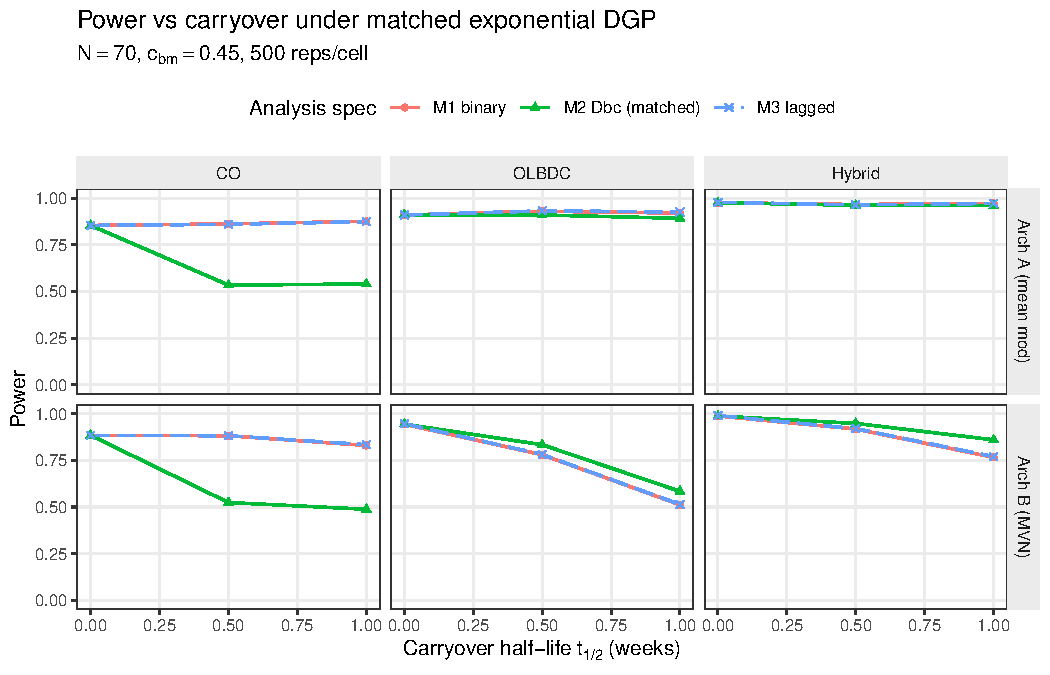
\includegraphics[width=0.9\linewidth]{../../figures/02-power-by-spec} \caption{Power versus carryover half-life under the exponential DGP, stratified by analysis specification. The matched specification M2 tracks closely with the nominally inferior M1 and M3 at low half-lives but retains a modest advantage at $t_{1/2} = 1.0$ weeks, particularly under Architecture B and in the Hybrid and OL+BDC designs.}\label{fig:fig-power-by-spec}
\end{figure}

\begin{bullets}

\textbf{Specifications coincide at zero carryover and diverge as it
grows, but M2's lead is confined to Architecture B's non-crossover
designs.}

\begin{itemize}\setlength{\itemsep}{2pt}\setlength{\parskip}{0pt}
\item All three are near-identical at $t_{1/2} = 0$.
\item M2's advantage emerges at $t_{1/2} = 0.5$ and grows under
Architecture B in the Hybrid and OL+BDC designs; M1 and M3 are
indistinguishable.
\item The advantage does not appear under the CO design (where M2 is
dominated) or under Architecture A.
\end{itemize}

\end{bullets}

\begin{rgt}
rgt to complete.

\end{rgt}

\begin{orig}
The three analysis specifications yield near-identical power at
\(t_{1/2} = 0\), where there is no carryover to model, and diverge
progressively as carryover half-life increases. The matched
specification M2 retains a modest but consistent advantage
specifically under Architecture\textasciitilde B in the Hybrid and OL+BDC designs,
where the advantage emerges at \(t_{1/2} = 0.5\) weeks and grows
through \(t_{1/2} = 1.0\) weeks; M1 and M3 are effectively
indistinguishable. This advantage is confined to those strata: it
does not appear under the crossover (CO) design, where M2 is in
fact dominated (Section 5), nor under Architecture\textasciitilde A. The figure
therefore shows that the M2 advantage, where present, is not an
artifact of the single reference cell, not that it holds
everywhere.

\end{orig}

\subsection{Decay-form mis-specification}\label{decay-form-mis-specification}

\begin{figure}
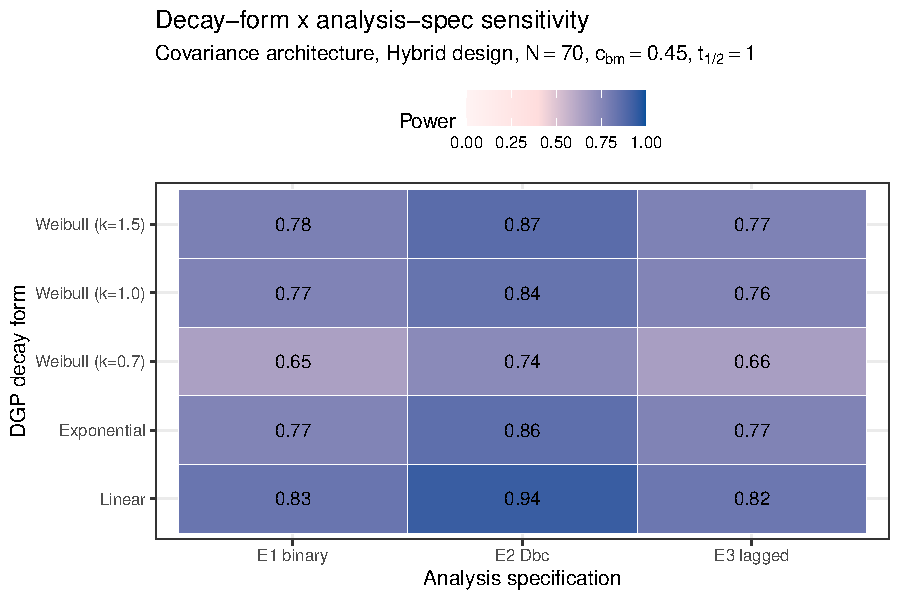
\includegraphics[width=0.7\linewidth]{../../figures/02-heatmap-matched-vs-mismatched} \caption{Power at the critical cell ($t_{1/2} = 1.0$ weeks, Architecture B, Hybrid design, $N = 70$, $c_{bm} = 0.45$) across DGP decay forms (rows) and analysis specifications (columns). Under the Weibull heavy-tailed DGP ($k = 0.7$) and the linear DGP, the exposure-weighted (M2) specification loses its advantage because its assumed exponential decay no longer matches truth.}\label{fig:fig-heatmap-mismatch}
\end{figure}

\begin{bullets}

\textbf{The heatmap separates two mis-specification directions:
wrong analysis given the DGP, and wrong assumed DGP.}

\begin{itemize}\setlength{\itemsep}{2pt}\setlength{\parskip}{0pt}
\item Matched reference (exp DGP $\times$ M2): power
$0.860 \pm 0.016$.
\item Same row, other columns: penalty of M1/M3 under an exponential
DGP.
\item M2 column, other rows: cost of assuming exponential when the
truth is linear or Weibull.
\end{itemize}

\end{bullets}

\begin{rgt}
rgt to complete.

\end{rgt}

\begin{orig}
The heatmap cell at the intersection of the exponential DGP row
and the M2 analysis column is the matched reference
(power \(0.860 \pm 0.016\)). Cells in the same row but other
columns quantify the power penalty of analyzing under the wrong
specification when the DGP is exponential; cells in the M2 column
but other rows quantify the cost of assuming exponential decay
in the analysis when the true DGP is linear or Weibull. The
Discussion (Section 5) takes up the practical interpretation of
both off-diagonal directions.

\end{orig}

\subsection{Type I error control and cluster-robust recalibration}\label{type-i-error-control-and-cluster-robust-recalibration}

\begin{figure}
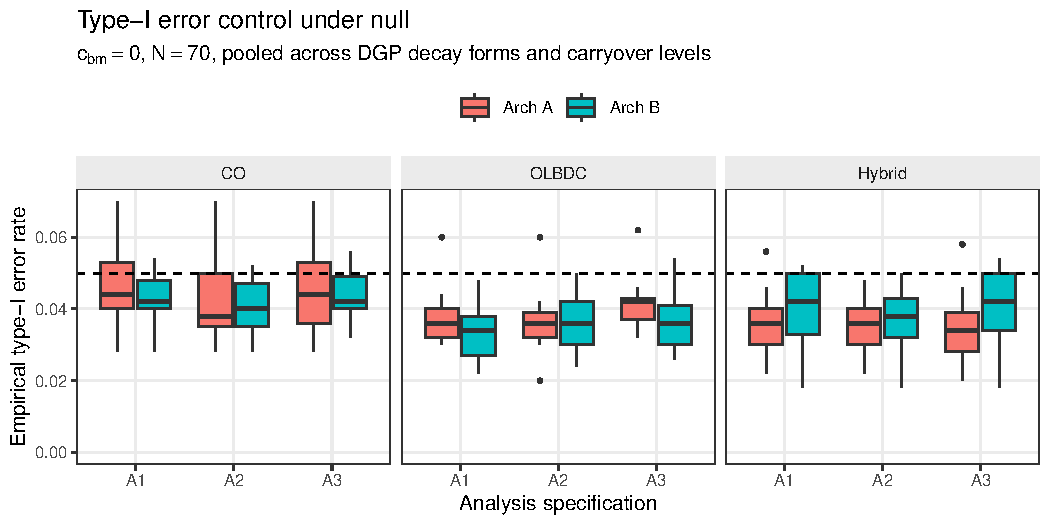
\includegraphics[width=0.95\linewidth]{../../figures/02-type1-boxplots} \caption{Empirical Type I error rates under the null ($c_{bm} = 0$), pooled across DGP decay forms and carryover half-lives, stratified by design and analysis specification. Boxplots cover the distribution across cells at $N = 70$; the dashed reference line marks the nominal 0.05 level.}\label{fig:fig-type1}
\end{figure}

\begin{bullets}

\textbf{Type I error is conservative (mean 0.039), reflecting the
corCAR1 working-covariance conservatism rather than inflation.}

\begin{itemize}\setlength{\itemsep}{2pt}\setlength{\parskip}{0pt}
\item Mean 0.039 across 540 null cells; cell maximum 0.084,
unremarkable under grid multiplicity (cells are not independent).
\item No specification or architecture inflates the rate above
nominal.
\item The companion study traces the shortfall to a 6-10\%
over-estimated SE; block S6's CR2 (below) restores nominal size
without changing the ranking.
\end{itemize}

\end{bullets}

\begin{rgt}
rgt to complete.

\end{rgt}

\begin{orig}
Mean empirical Type I error across all 540 null cells is 0.039,
below the nominal 0.05 level. The cell-level maximum is 0.084. This
exceeds the single-cell binomial 95\% interval \([0.031, 0.069]\) for
nominal 0.05 at \(n_{sim} = 500\), but is unremarkable once
multiplicity over the grid is acknowledged. We do not invoke an
exact maximum-order-statistic bound here, because the cells are not
independent: the three specifications within a cell share common
random numbers, and at \(t_{1/2} = 0\) the decay-form cells coincide.
The qualitative reading is unaffected -- no specification or
architecture inflates the rate above nominal, and the central
tendency is, if anything, conservative. That shortfall below
nominal is not sampling slack but the conservatism of the
model-based
interaction test that the companion calibration study\textsuperscript{\citeproc{ref-pmsimstats_calibration2026}{5}} traces to the corCAR1 working
covariance: its standard error is over-estimated by six to ten
percent and the realized rejection rate falls correspondingly.
The conservatism is uniform across specifications and
architectures, which is why it leaves the comparison intact;
the cluster-robust recalibration reported below (block S6) confirms
that a CR2 cluster-robust standard error restores the rejection rate
to nominal without disturbing the specification ranking. Table \ref{tab:tab-type1-cr2} makes the
per-specification conservatism and its cluster-robust correction
explicit at the null cell.

\end{orig}

\begin{table}

\caption{\label{tab:tab-type1-cr2}Conservatism of the model-based interaction test and its
    cluster-robust correction, at the null cell ($c_{bm} = 0$,
    exponential DGP, $t_{1/2} = 1.0$ weeks, Hybrid design, $N = 70$,
    Architecture B, 3{,}000 replicates). $\kappa$ is the ratio of the
    mean standard error to the empirical standard deviation of the
    interaction estimate; $\kappa > 1$ indicates a conservative test.
    Type I is the empirical rejection rate of
    $H_0: \beta_{bm:X} = 0$ at $\alpha = 0.05$, with Monte Carlo
    standard error about 0.004. All three specifications are
    conservative under the model-based test, most so the
    exposure-weighted M2 ($\kappa = 1.10$, Type I $= 0.029$); the CR2
    bias-reduced cluster-robust standard error restores $\kappa$ to
    near one and Type I to nominal (0.045 to 0.049) for every
    specification.}
\centering
\begin{tabular}[t]{lllll}
\toprule
Specification & $\kappa$ model & Type I model & $\kappa$ CR2 & Type I CR2\\
\midrule
M1 & 1.06 & 0.036 & 0.98 & 0.048\\
M2 & 1.10 & 0.029 & 1.00 & 0.045\\
M3 & 1.05 & 0.039 & 0.98 & 0.049\\
\bottomrule
\end{tabular}
\end{table}

\begin{bullets}

\textbf{Block S6 re-fits M2 with a CR2 cluster-robust SE to correct
the mild conservatism of the model-based test.}

\begin{itemize}\setlength{\itemsep}{2pt}\setlength{\parskip}{0pt}
\item The model-based SE is 6-10\% too large, so power figures are
slight under-estimates.
\item The CR2 sandwich does not trust the model's covariance
assumption and fixes the calibration.
\item Table \\ref{tab:tab-s6} checks reference and four stress cells.
\end{itemize}

\end{bullets}

\begin{rgt}
rgt to complete.

\end{rgt}

\begin{orig}
The companion calibration study\textsuperscript{\citeproc{ref-pmsimstats_calibration2026}{5}} shows
that this mixed-model test is mildly \textbf{conservative}: its standard
error is about 6-10\% too large, so it rejects a true effect a bit
less often than it should (this is why the null rejection rate above,
0.039, sits below 0.05, and why the power numbers are slight
under-estimates). A \textbf{cluster-robust standard error} (the CR2
estimator, which does not trust the model's covariance assumption)
fixes the calibration. Table \ref{tab:tab-s6} re-fits M2 with both
the model-based and the CR2 standard error at the reference cell and
four stress cells, to check that fixing the calibration does not
change the ranking.

\end{orig}

\begin{table}
\centering
\caption{\label{tab:tab-s6}Cluster-robust recalibration of the exposure-weighted
    specification M2 at the reference cell and four stress cells
    (500 replicates, $c_{bm} = 0.45$, Architecture B). $\kappa$ is the
    ratio of the mean standard error to the empirical standard
    deviation of the interaction estimate; a value above one is a
    conservative test. The M2$-$M1 columns give the power gap between
    the two specifications under each inference, a check that
    recalibration preserves the ranking. CR2 df is the mean
    Satterthwaite degrees of freedom for the cluster-robust test; the
    model-based test carries roughly 480. Computed with the
    \texttt{clubSandwich} package; see the companion calibration study
    for the mechanism. The S6 cells are an independent 500-replicate
    run, so the model-based M2 power at the reference cell (0.829)
    differs from the headline-grid value (0.860) by within one Monte
    Carlo standard error ($\approx 0.016$); the two should not be
    read as conflicting.}
\centering
\resizebox{\ifdim\width>\linewidth\linewidth\else\width\fi}{!}{
\begin{tabular}[t]{llllllll}
\toprule
Cell & $\kappa$ model & $\kappa$ CR2 & Power model & Power CR2 & M2$-$M1 model & M2$-$M1 CR2 & CR2 df\\
\midrule
Reference, $N=70$ & 1.15 & 0.99 & 0.829 & 0.863 & +0.080 & +0.092 & 23\\
Small $N=35$ & 1.13 & 0.96 & 0.558 & 0.590 & +0.066 & +0.086 & 12\\
High autocorr, $\rho=0.9$ & 1.26 & 0.94 & 0.954 & 0.980 & +0.052 & +0.032 & 23\\
Half-life mis-spec & 1.14 & 1.00 & 0.759 & 0.795 & +0.010 & +0.024 & 23\\
30\% MCAR dropout & 0.99 & 0.85 & 0.148 & 0.126 & +0.010 & +0.010 & 5\\
\bottomrule
\end{tabular}}
\end{table}

\begin{figure}
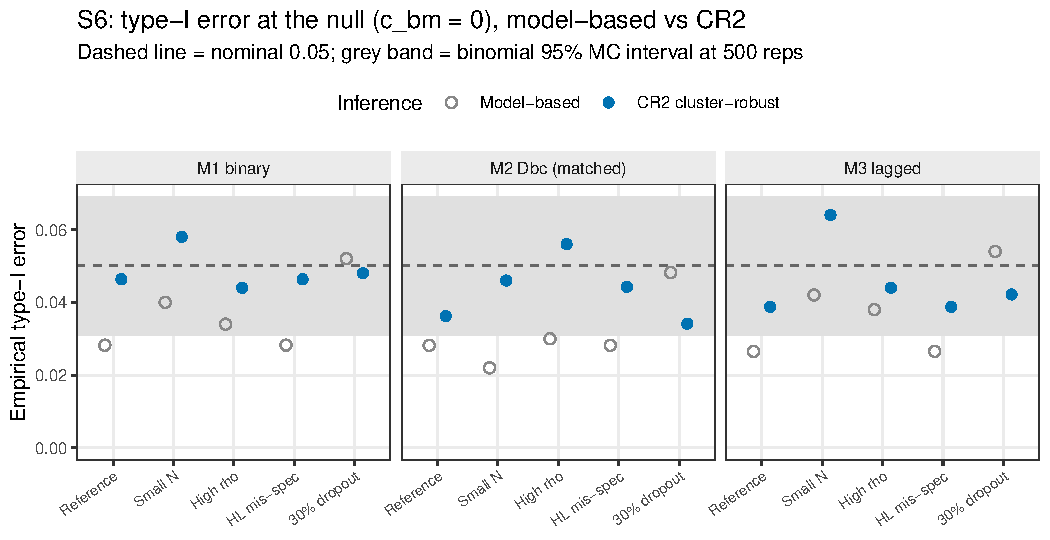
\includegraphics[width=0.95\linewidth]{../../figures/02-type1-cr2} \caption{Empirical Type I error at the null ($c_{bm} = 0$) under the model-based and CR2 cluster-robust inference, across the five S6 cells and the three specifications. The model-based test (open) is conservative (near 0.03); CR2 (filled) is restored to the nominal 0.05 (dashed), within the binomial Monte Carlo band (gray). 500 null replicates per cell.}\label{fig:fig-type1-cr2}
\end{figure}

\begin{bullets}

\textbf{CR2 restores nominal size, which is the precondition for
preferring any specification on power -- only correctly-sized tests
are comparable.}

\begin{itemize}\setlength{\itemsep}{2pt}\setlength{\parskip}{0pt}
\item Model-based null rejection sits near 0.03 (mean 0.035) across
all cells and specs -- the documented conservatism
(Fig. \\ref{fig:fig-type1-cr2}).
\item CR2 lifts it to a mean of 0.046, within the Monte Carlo band
around 0.05.
\item Under CR2 all three specifications hold nominal $\alpha$, so
the M2 advantage is a comparison among correctly-sized tests.
\end{itemize}

\end{bullets}

\begin{rgt}
rgt to complete.

\end{rgt}

\begin{orig}
The effect of recalibration on test size is shown directly in
Figure \ref{fig:fig-type1-cr2}: the model-based null rejection rate
sits near 0.03 (mean 0.035) across all five cells and three
specifications, while the CR2 test restores it to a mean of 0.046,
within the Monte Carlo band around the nominal 0.05. This is the
precondition for the whole comparison -- a test that is not
correctly sized cannot be preferred on power alone -- so under CR2,
where all three specifications hold nominal \(\alpha\), the M2
advantage is a like-for-like comparison among correctly-sized tests.

\end{orig}

\begin{bullets}

\textbf{CR2 restores calibration ($\kappa \to 1$) and recovers
power without changing the ranking, but only in information-rich
cells.}

\begin{itemize}\setlength{\itemsep}{2pt}\setlength{\parskip}{0pt}
\item $\kappa$ falls from 1.07-1.26 to about 1; the correctly-sized
test recovers two to five power points.
\item The M2$-$M1 gap is held or widened, at the cost of far fewer
degrees of freedom ($\approx 480 \to 23$).
\item Validated only at Architecture B / Hybrid / $N = 70$; do not
extend the lower-bound reading to CO or Architecture A.
\end{itemize}

\end{bullets}

\begin{rgt}
rgt to complete.

\end{rgt}

\begin{orig}
In the information-rich cells the picture matches the companion
study. The calibration ratio \(\kappa\) (mean standard error divided
by the true spread of the estimates; above 1 means conservative)
runs 1.07-1.26 under the model and is restored to about 1 under
CR2, and the correctly-sized test recovers two to five points of
power. Crucially, the M2-minus-M1 gap is held or slightly widened,
so \textbf{fixing the calibration does not change the ranking}. The
price is fewer effective degrees of freedom (about 480 drops to
\textasciitilde23). Under heavy dropout the trick stops helping: the model is no
longer conservative, CR2 becomes slightly anti-conservative on its
handful of degrees of freedom, and all methods have collapsed to
\textasciitilde0.13 power anyway. One caution: this recalibration was validated
only in the Architecture\textasciitilde B, Hybrid, \(N = 70\) cells, so the
``slightly conservative lower bound'' reading applies there, not to
the crossover design or Architecture\textasciitilde A where M2 does not lead.

\end{orig}

\subsection{Sensitivity analyses}\label{sensitivity-analyses}

\begin{bullets}

\textbf{Five Tier 2 blocks perturb one axis at a time around the
reference cell.}

\begin{itemize}\setlength{\itemsep}{2pt}\setlength{\parskip}{0pt}
\item Reference: Architecture B, Hybrid, $N = 70$, $c_{bm} = 0.45$,
exponential DGP, $t_{1/2} = 1.0$.
\item Each block varies one axis with the others held fixed.
\item Blocks are reported separately, not pooled with Tier 1 or each
other.
\end{itemize}

\end{bullets}

\begin{rgt}
rgt to complete.

\end{rgt}

\begin{orig}
Before going into the individual blocks, we note the general
design. Five Tier 2 marginal sensitivity blocks probe the
robustness of the Tier 1 ranking to single-axis perturbations
around the reference configuration (Architecture B, Hybrid
design, \(N = 70\), \(c_{bm} = 0.45\), exponential DGP,
\(t_{1/2} = 1.0\) weeks). Each block varies one axis and holds the
others at their reference values. Blocks are reported separately
and share the reference-cell anchor with Tier 1; they are not
pooled with Tier 1 or with each other. The design rationale is
documented in
\texttt{analysis/scripts/carryover-sensitivity/simulation-grid-plan.md}.

\end{orig}

\subsubsection{S1: within-factor autocorrelation}\label{s1-within-factor-autocorrelation}

\begin{figure}
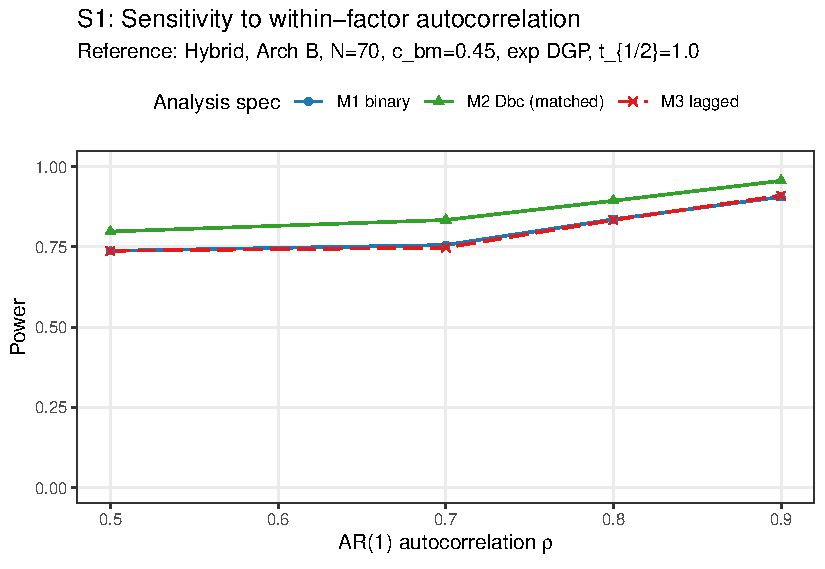
\includegraphics[width=0.7\linewidth]{../../figures/02-sens-S1} \caption{Power by analysis specification across AR(1) autocorrelation $\rho \in \{0.5, 0.7, 0.8, 0.9\}$. Hendrickson (2020) uses $\rho = 0.8$; docs/02 uses $\rho = 0.7$ after positive-definiteness reductions.}\label{fig:fig-sens-s1}
\end{figure}

\begin{bullets}

\textbf{S1: autocorrelation lifts all three specifications equally,
preserving M2's $\approx 0.06$ advantage at every $\rho$.}

\begin{itemize}\setlength{\itemsep}{2pt}\setlength{\parskip}{0pt}
\item Power rises monotonically with $\rho$ for all three.
\item M2's advantage holds near 0.06 across $\rho \in [0.5, 0.9]$.
\item Autocorrelation and the specification act additively, not
multiplicatively.
\end{itemize}

\end{bullets}

\begin{rgt}
rgt to complete.

\end{rgt}

\begin{orig}
All three specifications gain power monotonically with \(\rho\).
At \(\rho = 0.5\), M2 power is \(0.798 \pm 0.018\) versus M1
\(0.738 \pm 0.020\) and M3 \(0.738 \pm 0.020\); at \(\rho = 0.9\),
M2 reaches \(0.956 \pm 0.009\) versus M1 \(0.906 \pm 0.013\) and
M3 \(0.910 \pm 0.013\) (point estimate \(\pm\) MCSE,
\(n_{sim} = 500\)). Contrary to the prior expectation that M2
would be the most \(\rho\)-sensitive specification, all three
exhibit comparable relative gains across the explored range.
The M2 advantage over M1 and M3, approximately 0.06 in absolute
power throughout, is preserved at every AR(1) level. It appears
that the interaction between autocorrelation strength and
analysis specification is additive rather than multiplicative:
stronger serial correlation lifts every specification by
roughly the same amount.

\end{orig}

\subsubsection{S2: analyst-truth half-life mismatch}\label{s2-analyst-truth-half-life-mismatch}

\begin{figure}
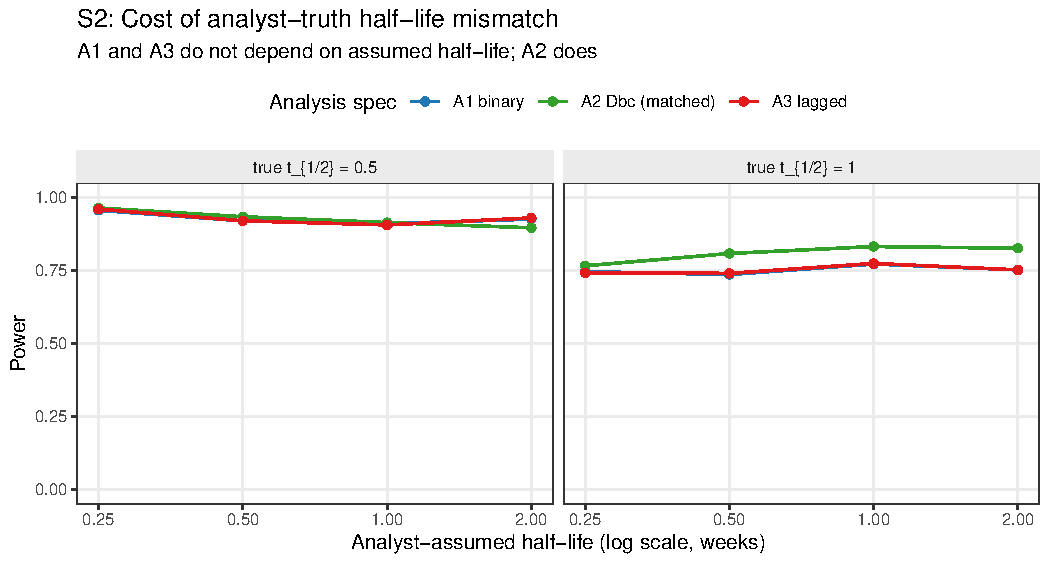
\includegraphics[width=0.9\linewidth]{../../figures/02-sens-S2} \caption{Power of M1, M2, and M3 as the analyst's assumed half-life departs from the true DGP half-life. M1 and M3 are invariant to the assumed half-life by construction; M2's power degrades with mis-specification.}\label{fig:fig-sens-s2}
\end{figure}

\begin{bullets}

\textbf{S2: M2 keeps its advantage even when the assumed half-life
is wrong by a factor of two or four.}

\begin{itemize}\setlength{\itemsep}{2pt}\setlength{\parskip}{0pt}
\item M2 averages 0.868 over eight assumed/true half-life cells
(range 0.766-0.964).
\item M1 and M3 are invariant to the assumed half-life (average
0.840).
\item M2's gentle curvature makes it a defensible default under an
approximately-known half-life.
\end{itemize}

\end{bullets}

\begin{rgt}
rgt to complete.

\end{rgt}

\begin{orig}
M2 is markedly more robust to analyst-truth half-life mismatch
than the prior expectation predicted. Across the eight S2 cells
(DGP \(t_{1/2} \in \{0.5, 1.0\}\) weeks crossed with analyst-assumed
\(t_{1/2} \in \{0.25, 0.5, 1.0, 2.0\}\) weeks), M2 averages 0.868,
ranging from 0.766 (DGP 1.0 weeks analyzed at 0.25 weeks) to
0.964 (DGP 0.5 weeks analyzed at 0.25 weeks); per-cell MCSE
ranges from 0.008 to 0.019. M1 and M3 are invariant to the
analyst-assumed half-life by construction, as they do not consume
the parameter, and their power averages 0.840 each across the same
eight cells. The exposure-weighted predictor's curvature is
sufficiently gentle that mis-specification of the assumed
half-life by a factor of two does not erode M2's advantage over
M1 and M3 at either DGP half-life. The result suggests that the
exposure-weighted (M2) specification is a defensible default even when the
true pharmacokinetic half-life is only approximately known at the
design stage.

\end{orig}

\subsubsection{S3: dropout}\label{s3-dropout}

\begin{figure}
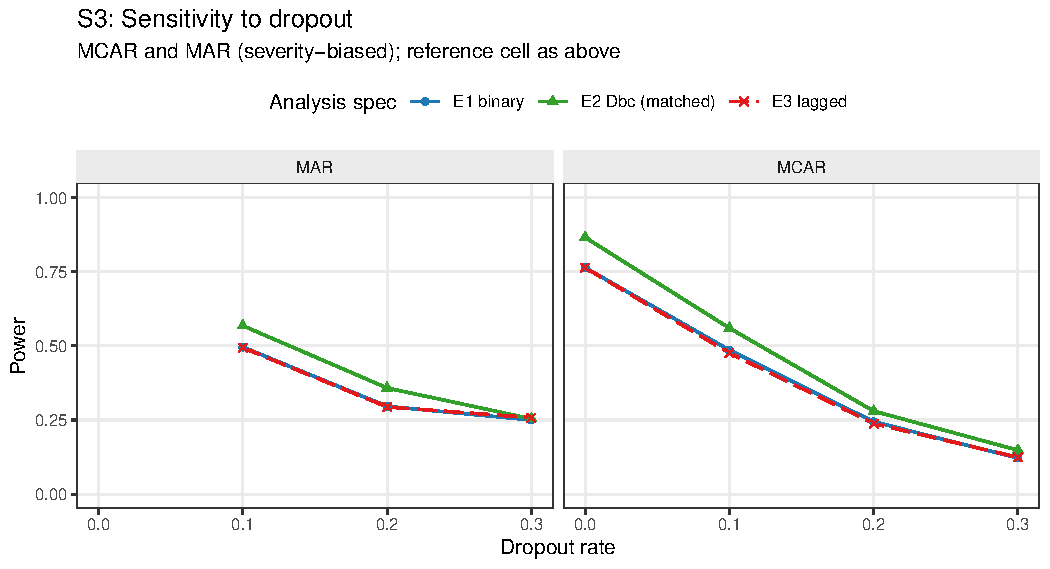
\includegraphics[width=0.9\linewidth]{../../figures/02-sens-S3} \caption{Power at dropout rates $\in \{0, 0.1, 0.2, 0.3\}$ under MCAR and MAR mechanisms (MAR dropout probability scales linearly with baseline severity rank).}\label{fig:fig-sens-s3}
\end{figure}

\begin{bullets}

\textbf{S3: dropout collapses power for all three methods, and
narrows M2's advantage as off-drug observations are dropped.}

\begin{itemize}\setlength{\itemsep}{2pt}\setlength{\parskip}{0pt}
\item At 30\% missing-completely-at-random (MCAR) dropout all three fall to about 0.12-0.15, effectively
tied.
\item The M2$-$M1 gap shrinks from $\approx 0.10$ (no dropout) to
$\approx 0.03$ (30\% MCAR).
\item M2's signal lives in off-drug points, so dropping them erodes
its edge; the advantage survives at dropout $\leq 0.20$.
\end{itemize}

\end{bullets}

\begin{rgt}
rgt to complete.

\end{rgt}

\begin{orig}
All three specifications lose power monotonically with dropout
rate. The MCAR baseline (\(N = 70\), dropout = 0) gives M1
\(0.764 \pm 0.019\), M2 \(0.866 \pm 0.015\), M3 \(0.764 \pm 0.019\);
at MCAR rate 0.30 these collapse to M1 \(0.122 \pm 0.015\), M2
\(0.148 \pm 0.016\), M3 \(0.124 \pm 0.015\). M2's advantage narrows
under heavy dropout: the absolute M2\(-\)M1 gap is approximately
0.10 at zero dropout, 0.07 at rate 0.10, 0.04 at rate 0.20, and
0.03 at rate 0.30 under MCAR. Under missing-at-random (MAR)
dropout with the same marginal
rate the gap narrows further at the highest rate (M2\(-\)M1
\(\approx 0.004\) at rate 0.30 MAR). The pattern is consistent
with the exposure-weighted (M2) specification's signal source residing in
the exposure-weighted contrast contributed by off-drug
observations: when those observations are preferentially
dropped, M2's advantage contracts toward M1's. At
low-to-moderate dropout (rate \(\leq 0.20\)) the M2 advantage is
preserved.

\end{orig}

\subsubsection{S4: biomarker-moderation effect-size curve}\label{s4-biomarker-moderation-effect-size-curve}

\begin{figure}
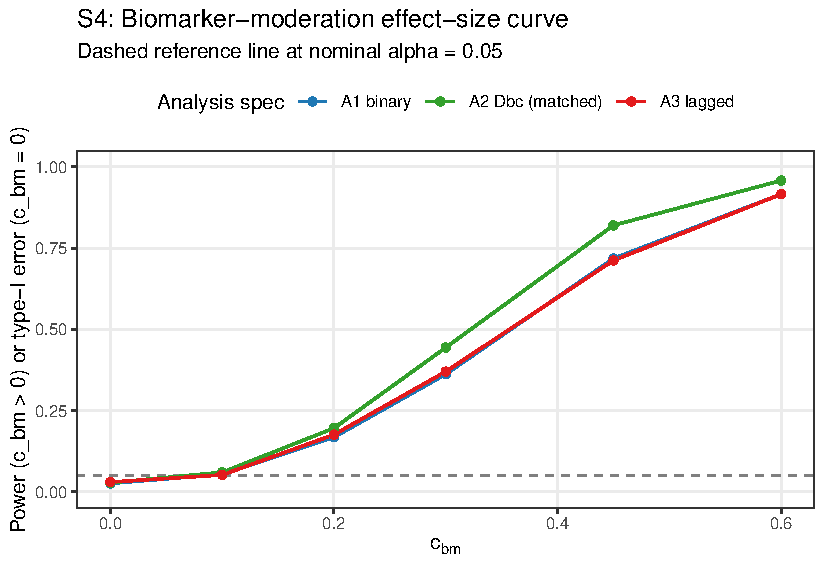
\includegraphics[width=0.7\linewidth]{../../figures/02-sens-S4} \caption{Power across the biomarker-moderation effect-size range $c_{bm} \in \{0, 0.10, 0.20, 0.30, 0.45, 0.60\}$ under Architecture B. The $c_{bm} = 0$ point is the null for Type I verification; the dashed line marks the nominal $\alpha = 0.05$.}\label{fig:fig-sens-s4}
\end{figure}

\begin{bullets}

\textbf{S4: the power curve is sigmoidal; M2's advantage peaks at
intermediate effect sizes and vanishes toward the ceiling.}

\begin{itemize}\setlength{\itemsep}{2pt}\setlength{\parskip}{0pt}
\item Type I error at $c_{bm} = 0$ is conservative (0.026-0.030).
\item M2$-$M1 peaks at $+0.102$ at $c_{bm} = 0.45$, shrinking to
$+0.042$ at $c_{bm} = 0.60$.
\item The advantage matters most for moderate
biomarker-treatment interactions.
\end{itemize}

\end{bullets}

\begin{rgt}
rgt to complete.

\end{rgt}

\begin{orig}
The expected sigmoidal power curve is observed across all three
specifications. At \(c_{bm} = 0\), empirical Type I error is below
the nominal level at \(0.026 \pm 0.007\) (M1), \(0.028 \pm 0.007\)
(M2), and \(0.030 \pm 0.008\) (M3); the conservative behavior is
consistent with the AR(1) reference distribution at moderate
sample sizes. Power rises through the mid-range and saturates at
\(c_{bm} \geq 0.45\): at \(c_{bm} = 0.6\), M1 reaches
\(0.916 \pm 0.012\), M2 \(0.958 \pm 0.009\), and M3
\(0.916 \pm 0.012\). The M2 advantage over M1 is largest at
intermediate effect sizes, \(+0.082\) absolute at \(c_{bm} = 0.30\)
(\(0.444\) versus \(0.362\)) and \(+0.102\) at \(c_{bm} = 0.45\)
(\(0.820\) versus \(0.718\)), shrinking to \(+0.042\) at \(c_{bm} = 0.60\)
where all specifications approach ceiling. The M2 advantage is
therefore most practically consequential in designs targeting
moderate biomarker-treatment interactions.

\end{orig}

\subsubsection{S5: autocorrelation by carryover (exploratory)}\label{s5-autocorrelation-by-carryover-exploratory}

\begin{figure}
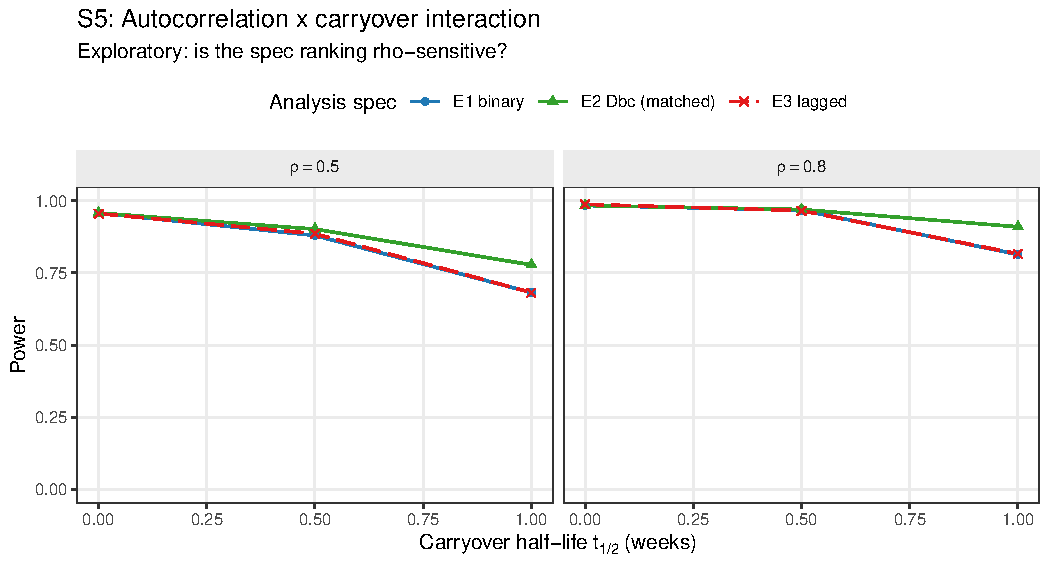
\includegraphics[width=0.9\linewidth]{../../figures/02-sens-S5} \caption{Power across carryover half-lives at $\rho \in \{0.5, 0.8\}$, by analysis specification. This block tests whether the $\rho$-sensitivity of the M1/M2/M3 ranking depends on carryover strength.}\label{fig:fig-sens-s5}
\end{figure}

\begin{bullets}

\textbf{S5: the M2 advantage is constant across the
$\rho \times t_{1/2}$ grid, confirming additive (not interactive)
effects.}

\begin{itemize}\setlength{\itemsep}{2pt}\setlength{\parskip}{0pt}
\item M2$-$M1 $= 0.096$ at both $\rho = 0.5$ and $\rho = 0.8$ when
$t_{1/2} = 1.0$.
\item Autocorrelation and carryover act additively on the ranking.
\item S5 reassures that the Tier 1 ranking holds across the grid.
\end{itemize}

\end{bullets}

\begin{rgt}
rgt to complete.

\end{rgt}

\begin{orig}
The M2 \(>\) M1 \(\approx\) M3 ranking is invariant to the
\(\rho \times t_{1/2}\) interaction. At \(\rho = 0.5\),
\(t_{1/2} = 1.0\) weeks, M2 \(-\) M1 = 0.096 (M2 \(0.778 \pm 0.019\),
M1 \(0.682 \pm 0.021\)); at \(\rho = 0.8\), \(t_{1/2} = 1.0\) weeks,
M2 \(-\) M1 = 0.096 (M2 \(0.910 \pm 0.013\), M1 \(0.814 \pm 0.017\)).
The absolute M2 advantage is constant across the
\(\rho \times t_{1/2}\) space, indicating that autocorrelation and
carryover strength act additively on the specification ranking
rather than interactively. Block S5 therefore functions as a
methodological reassurance: the Tier 1 ranking is preserved at
every level of \(\rho\) and \(t_{1/2}\) in the explored grid.

\end{orig}

\subsection{A higher-precision check}\label{a-higher-precision-check}

\begin{bullets}

\textbf{A higher-precision paired-McNemar rerun confirms M2's lead
is real (p $= 6.6 \times 10^{-17}$ at the strongest cell).}

\begin{itemize}\setlength{\itemsep}{2pt}\setlength{\parskip}{0pt}
\item 24-cell OL+BDC rerun at 600 trials/cell, all converging.
\item Paired McNemar (same trials) at $N = 70$, half-life 1.0: M2
beats M1 by 13.7 points, $p = 6.6 \times 10^{-17}$.
\item M3 recovers only part of M2's advantage; Type I stayed within
$[0.003, 0.053]$.
\end{itemize}

\end{bullets}

\begin{rgt}
rgt to complete.

\end{rgt}

\begin{orig}
Because some of these gaps are small, we reran a focused 24-cell
grid (the OL+BDC design, \(N \in \{35, 70\}\), true half-life \(\in
\{0.5, 1.0\}\)) at 600 trials per cell, all converging. Because the
three methods see the \emph{same} trials, we can compare them with a
paired \textbf{McNemar test}, which counts only the trials where two
methods disagree -- a much more sensitive comparison than treating
the methods as independent. At the strongest cell (\(N = 70\), true
half-life 1.0) M2 beats M1 by 13.7 points (0.737 vs 0.873) with
McNemar \(p = 6.6 \times 10^{-17}\): the lead is real, not noise. The
shape-free method M3 recovers only part of M2's advantage, and only
at small \(N\) and short half-life; at larger \(N\) it captures about
half. Type I error across the null cells stayed in \([0.003, 0.053]\),
i.e.~at or below the nominal 5\%.

\end{orig}

\section{Discussion}\label{discussion}

\subsection{The main result, and where it breaks down}\label{the-main-result-and-where-it-breaks-down}

\begin{bullets}

\textbf{M2's advantage is real but conditional: highest in only
19\% of cells, dominated under CO and under Architecture A.}

\begin{itemize}\setlength{\itemsep}{2pt}\setlength{\parskip}{0pt}
\item Best cell (Arch B, Hybrid): M2 beats M1/M3 by $\approx 10$
points ($\approx 5$ MCSEs).
\item M2 is the best method in only 68 of 360 non-null cells; under
CO it is much worse (0.488 vs 0.830).
\item Mechanism: the crossover's within-subject correlation already
carries the signal M2 targets, so M2 only loses there.
\end{itemize}

\end{bullets}

\begin{rgt}
rgt to complete.

\end{rgt}

\begin{orig}
The headline is that M2's advantage is real but \textbf{conditional}.
At its best cell (Architecture B, Hybrid design, \(N = 70\),
\(c_{bm} = 0.45\), \(t_{1/2} = 1.0\)) M2 beats M1 and M3 by about 10
percentage points of power (0.860 vs 0.766 and 0.770) -- about five
MCSEs, so not luck. But M2 is the best method
in only 68 of the 360 cells with a real effect (19\%). In the
crossover design it is much \emph{worse} (0.488 vs 0.830 for M1), and
under Architecture A it is slightly worse everywhere. There is a
clean reason for the crossover failure: in a crossover the
within-subject correlation already carries most of the signal that
M2's decaying predictor is designed to recover, so M2 has nothing
left to gain and its down-weighting of off-drug points only hurts.
The ranking ``M2 best'' therefore holds only under Architecture B in
the two non-crossover designs.

\end{orig}

\subsection{What the robustness checks add}\label{what-the-robustness-checks-add}

\begin{bullets}

\textbf{Where M2 leads, the lead survives all three robustness
checks.}

\begin{itemize}\setlength{\itemsep}{2pt}\setlength{\parskip}{0pt}
\item Decay shape: M2 never drops below M1/M3 even when the assumed
form is wrong (worst case the linear truth).
\item Assumed half-life: a two- to four-fold error moves M2 only
from 0.83 to 0.77, never below M1/M3.
\item Autocorrelation: lifts all three equally, so M2's 5-6 point
lead is $\rho$-independent.
\end{itemize}

\end{bullets}

\begin{rgt}
rgt to complete.

\end{rgt}

\begin{orig}
Three checks probe whether M2's win, where it exists, is fragile.
\textbf{Decay shape (Fig. \ref{fig:fig-heatmap-mismatch}).} Even when
the analyst wrongly assumes exponential decay but the truth is
linear or Weibull, M2 still does not drop below M1 or M3; the worst
case is the linear truth, whose sharp cutoff is hardest to
approximate. \textbf{Assumed half-life (Fig. \ref{fig:fig-sens-s2}).}
M1 and M3 do not use a half-life, so they are unaffected; M2 does,
yet getting the half-life wrong by a factor of two or four moves
its power only from about 0.83 to 0.77, never below M1/M3. So M2 is
forgiving of a roughly-guessed half-life. \textbf{Autocorrelation
(Fig. \ref{fig:fig-sens-s1}).} Stronger serial correlation raises
all three methods by about the same amount, so M2's lead stays near
5-6 points and does not depend on the correlation strength.

\end{orig}

\subsection{Dropout matters more than the method}\label{dropout-matters-more-than-the-method}

\begin{bullets}

\textbf{Dropout collapses power for all methods equally, so it
dominates the specification choice.}

\begin{itemize}\setlength{\itemsep}{2pt}\setlength{\parskip}{0pt}
\item At 30\% dropout all three fall to 0.12-0.25 and become
indistinguishable.
\item MAR (severity-related) dropout is slightly worse than MCAR,
because the highest-signal patients leave first.
\item Keeping patients in the trial buys more power than any
carryover method.
\end{itemize}

\end{bullets}

\begin{rgt}
rgt to complete.

\end{rgt}

\begin{orig}
The most sobering result is about \emph{missing data}, not carryover.
When patients drop out (Fig. \ref{fig:fig-sens-s3}), power
collapses for all three methods together: at 30\% dropout every
method falls to 0.12-0.25 and they become indistinguishable. M2
cannot protect against the loss; it only organizes whatever data
remain. Dropout that is related to severity (MAR) is slightly worse
than purely random dropout (MCAR), because the sickest patients --
who carry the most signal -- leave first. The practical message is
blunt: keeping patients in the trial buys far more power than any
choice of carryover method.

\end{orig}

\subsection{Architecture dependence}\label{architecture-dependence}

\begin{bullets}

\textbf{M2's advantage exists only under Architecture B, because
only there does carryover erode a correlation for M2 to recover.}

\begin{itemize}\setlength{\itemsep}{2pt}\setlength{\parskip}{0pt}
\item Architecture B is more carryover-sensitive under every decay
form and Weibull shape.
\item Under Architecture A, M2 is marginally negative everywhere
(e.g.\ Hybrid, $t_{1/2} = 1.0$: 0.960 vs M1 0.972).
\item Under A the effect stays proportional, so there is no
attenuated correlation to recover and the binary M1 is preferable.
\end{itemize}

\end{bullets}

\begin{rgt}
rgt to complete.

\end{rgt}

\begin{orig}
The companion manuscript establishes that Architecture B (MVN
differential correlation) loses substantially more power under
carryover than Architecture A (direct mean moderation). The
present results confirm that this qualitative gap is robust to
decay-form variation: Architecture B is more sensitive to
carryover under all three decay forms and at all five Weibull
shape values examined. The M2 advantage, however, is confined to
Architecture B: under Architecture A it is marginally negative in
every design (for example, at the Hybrid cell, \(t_{1/2} = 1.0\)
weeks, M2 = 0.960 versus M1 = 0.972). This is consistent with the
mechanism. Under Architecture B, carryover erodes the
biomarker-response correlation directly, and the continuous
exposure-weighted predictor recovers more of that attenuated
signal than either the binary on-drug indicator or the
lagged-nuisance term can; under Architecture A the treatment
effect remains proportional at every timepoint, so there is no
attenuated correlation for the exposure-weighted predictor to
recover and the simpler binary indicator is marginally preferable.
The M2 \(>\) M1 \(\approx\) M3 ranking therefore holds under
Architecture B in the non-crossover designs but not under
Architecture A, a dependence that trialists must weigh against the
assumed data-generating mechanism.

\end{orig}

\subsection{How this fits with earlier work, and its limits}\label{how-this-fits-with-earlier-work-and-its-limits}

\begin{bullets}

\textbf{Our results reproduce Hendrickson and engage the
crossover, variance-component, and carryover-testing literatures.}

\begin{itemize}\setlength{\itemsep}{2pt}\setlength{\parskip}{0pt}
\item M2 power 0.860 reproduces Hendrickson's 0.82; the new content
is the M1/M2/M3 comparison.
\item The Jones-Kenward expectation that a shape-free M3 beats M2
under mis-specification is not supported here.
\item Senn's variance-component view matches the additive
autocorrelation effect; Sturdevant-Lumley address the complementary
carryover-testing problem.
\end{itemize}

\end{bullets}

\begin{rgt}
rgt to complete.

\end{rgt}

\begin{orig}
Our matched-decay (M2) power at the headline cell, \(0.860 \pm
0.016\), reproduces Hendrickson's\textsuperscript{\citeproc{ref-hendrickson2020}{2}} reported 0.82
for the same cell; the new content is the head-to-head comparison
of M1, M2, and M3, which Hendrickson did not do. The crossover
tradition of Jones and Kenward\textsuperscript{\citeproc{ref-jones2014crossover}{4}} predicted
that a shape-free lagged term (M3) should beat a parametric
predictor (M2) when the decay shape is guessed wrong; our S2 result
does not support this in the range we tested, because M2's penalty
for a wrong half-life is too small for M3 to overtake it. Senn's\textsuperscript{\citeproc{ref-senn2016mastering}{6}} variance-component reasoning is consistent
with our finding that autocorrelation lifts all methods together.
A related but distinct strand, exemplified by Sturdevant and Lumley\textsuperscript{\citeproc{ref-sturdevant2021carryover}{7}}, develops mixed-effects \emph{tests for
carryover} after treatment cessation; our concern is the
complementary one of how carryover, once present, degrades the
biomarker-interaction test, but their work reinforces that
carryover is a first-order inferential issue in within-subject
designs rather than a nuisance to be assumed away.

\end{orig}

\begin{bullets}

\textbf{Two limitations: a single parameter set, and one-factor-at-
a-time sensitivity checks.}

\begin{itemize}\setlength{\itemsep}{2pt}\setlength{\parskip}{0pt}
\item Numbers come from one prazosin/PTSD parameterization, so
absolute power values are illustrative; the ranking is the portable
part.
\item The sensitivity blocks vary one factor at a time and can miss
factor interactions.
\item The one joint check (S5) showed no surprises.
\end{itemize}

\end{bullets}

\begin{rgt}
rgt to complete.

\end{rgt}

\begin{orig}
Two limitations bound these conclusions. First, the numbers come
from one parameter set (calibrated to a prazosin/PTSD trajectory),
so the \emph{absolute} power values are illustrative; the \emph{ranking} is
the portable part, and even it is conditional on the architecture
and design as shown above. Second, the sensitivity checks vary one
factor at a time, so they can miss interactions between factors
(for example, high autocorrelation combined with heavy dropout);
the one joint check we ran, S5, showed no surprises.

\end{orig}

\section{Conclusions}\label{conclusions}

\begin{enumerate}
\def\labelenumi{\arabic{enumi}.}
\item
  \textbf{M2 helps, but only conditionally.} The exposure-weighted
  predictor gives the highest power -- about 10 points over M1 --
  \emph{only} under Architecture B in the Hybrid and OL+BDC designs,
  and the lead survives wrong decay-shape and wrong half-life
  assumptions there. Under the crossover design, or under
  Architecture A, M2 has no advantage and M1 is at least as good.
  Where M2 is used, report it with a CR2 cluster-robust standard
  error (Section on Block S6).
\item
  \textbf{A guessed half-life is fine (where M2 is used).} Getting the
  half-life wrong by a factor of two to four barely moves M2's
  power, so a rough pharmacokinetic estimate suffices.
\item
  \textbf{The shape-free method M3 is essentially M1.} Because its
  lagged term is only a nuisance control, M3 tracks M1 closely and
  never overtakes M2 in the settings we tested.
\item
  \textbf{Dropout beats everything.} Power falls sharply as dropout
  rises (about half lost at 20\% dropout), the same for all three
  methods. Preventing dropout matters more than the carryover
  method.
\item
  \textbf{The test is slightly conservative, and fixable.} All methods
  reject a little less than the nominal 5\% under the null; this is
  a known property of the working-covariance model, and the CR2
  cluster-robust standard error restores the correct rate while
  recovering a few points of power, without changing the ranking
  (Block S6).
\end{enumerate}

\section*{Notes and reproducibility}\label{notes-and-reproducibility}
\addcontentsline{toc}{section}{Notes and reproducibility}

The authors declare no conflicts of interest and received no
specific funding. All data and code are in the pmsimstats-ng
project repository: cell-level summaries at
\texttt{analysis/data/02-grid-summary.rds} and \texttt{02-sensitivity-summary.rds},
drivers under \texttt{analysis/scripts/carryover-sensitivity/}, and the
pre-registered grid plan at \texttt{simulation-grid-plan.md}. The
manuscript loads pre-computed summaries only; no simulation runs
during knitting. The production simulation ran under R 4.5.3 and
the document is rendered under R 4.6.0, both pinned via \texttt{renv.lock}.

\section{References}\label{references}

\protect\phantomsection\label{refs}
\begin{CSLReferences}{0}{1}
\bibitem[\citeproctext]{ref-morris2019simulation}
\CSLLeftMargin{1. }%
\CSLRightInline{Morris TP, White IR, Crowther MJ. Using simulation studies to evaluate statistical methods. \emph{Statistics in Medicine}. 2019;38(11):2074-2102. doi:\href{https://doi.org/10.1002/sim.8086}{10.1002/sim.8086}}

\bibitem[\citeproctext]{ref-hendrickson2020}
\CSLLeftMargin{2. }%
\CSLRightInline{Hendrickson RC, Thomas RG, Schork NJ, Raskind MA. Optimizing aggregated {N}-of-1 trial designs for predictive biomarker validation: Statistical methods and practical considerations. \emph{Frontiers in Digital Health}. 2020;2:13. doi:\href{https://doi.org/10.3389/fdgth.2020.00013}{10.3389/fdgth.2020.00013}}

\bibitem[\citeproctext]{ref-pmsimstats_dgp_architectures2026}
\CSLLeftMargin{3. }%
\CSLRightInline{{pmsimstats team}. Two architectures for simulating biomarker-treatment interactions in aggregated {N}-of-1 trials. Published online 2026.}

\bibitem[\citeproctext]{ref-jones2014crossover}
\CSLLeftMargin{4. }%
\CSLRightInline{Jones B, Kenward MG. \emph{Design and Analysis of Cross-over Trials}. 3rd ed. CRC Press; 2014.}

\bibitem[\citeproctext]{ref-pmsimstats_calibration2026}
\CSLLeftMargin{5. }%
\CSLRightInline{{pmsimstats team}. Type-{I} calibration of fixed-effect interaction tests in linear mixed models: A staged diagnosis of working-covariance mis-specification and a cluster-robust remedy. Published online 2026.}

\bibitem[\citeproctext]{ref-senn2016mastering}
\CSLLeftMargin{6. }%
\CSLRightInline{Senn S. Mastering variation: Variance components and personalised medicine. \emph{Statistics in Medicine}. 2016;35(7):966-977. doi:\href{https://doi.org/10.1002/sim.6739}{10.1002/sim.6739}}

\bibitem[\citeproctext]{ref-sturdevant2021carryover}
\CSLLeftMargin{7. }%
\CSLRightInline{Sturdevant SG, Lumley T. Statistical methods for testing carryover effects: A mixed effects model approach. \emph{Contemporary Clinical Trials Communications}. 2021;22:100711. doi:\href{https://doi.org/10.1016/j.conctc.2021.100711}{10.1016/j.conctc.2021.100711}}

\end{CSLReferences}

\vfill

\begin{center}\rule{0.5\linewidth}{0.5pt}\end{center}

\emph{Rendered on 2026-07-30 at 14:06 PDT.}\\
\emph{Source: \texttt{\textasciitilde{}/prj/res/36-pmsimstats-ng/pmsimstats-ng/analysis/report/02-carryover-sensitivity/report-slim.Rmd}}

\end{document}
